\documentclass[11pt, letterpaper]{article}
%\documentclass{statsoc}
%\documentclass[aos]{imsart}
%\pdfminorversion=4
\pdfoutput=1
% NOTE: To produce blinded version, replace "0" with "1" below.
\newcommand{\blind}{1}

% DON'T change margins - should be 1 inch all around.
\addtolength{\evensidemargin}{-.5in}
\addtolength{\oddsidemargin}{-.5in}
\addtolength{\textwidth}{0.9in}
\addtolength{\textheight}{0.9in}
\addtolength{\topmargin}{-.4in}

% put your definitions there:
\usepackage{amsfonts}
\usepackage{amsmath}
\usepackage{amsthm}
\usepackage{bibentry}
\usepackage{color}
\usepackage{epsfig}
%\usepackage{float}
\usepackage{framed}
\usepackage{graphics}
\usepackage{hyperref}
\hypersetup{ colorlinks = true, citecolor = blue, urlcolor = blue}
\usepackage[utf8]{inputenc}
\usepackage[left, modulo]{lineno}
\usepackage{lmodern}
\usepackage{multirow}
%\usepackage{pdflscape}
%\usepackage{pdfpages}
\usepackage{relsize}
\usepackage{rotating}
\usepackage{subfigure}
\usepackage{subfiles}
\usepackage{url}
\usepackage{verbatim}
\usepackage{wrapfig}
\usepackage{floatrow}
% Table float box with bottom caption, box width adjusted to content
\newfloatcommand{capbtabbox}{table}[][\FBwidth]

\usepackage[round]{natbib}
% for algorithm
\usepackage[noend]{algpseudocode}
\usepackage{algorithm}
%\linenumbers

\usepackage{graphicx,psfrag,epsf}
\usepackage{enumerate}

\makeatletter
\@addtoreset{equation}{section}   % Makes \section reset 'equation' counter.
\renewcommand{\theequation}{\thesection.\arabic{equation}}
\makeatother

\makeatletter
\@addtoreset{figure}{section}
\renewcommand{\thefigure}{\thesection.\@arabic\c@figure}
\makeatother

\makeatletter
\@addtoreset{table}{section}
\renewcommand\thetable{\thesection.\@arabic\c@table}
\makeatother

%\theoremstyle{definition}
%\newtheorem{Example}{Example}[section]
%
%\theoremstyle{definition}
%\newtheorem{Remark}{Remark}[section]

\makeatletter
\newenvironment{Proof}[1][\proofname]{\par
  \normalfont
  \topsep6\p@\@plus6\p@ \trivlist
  \item[\hskip\labelsep\bfseries
    #1:]\ignorespaces
}{%
  \qed\endtrivlist
}
\makeatother

\usepackage{mycommands2}
\theoremstyle{definition}
\newtheorem{Algorithm}{Algorithm}
\newtheorem{Example}{Example}[section]
%\renewcommand{\baselinestretch}{1.25}
%\endlocaldefs
%\pdfminorversion=4

\begin{document}

\def\spacingset#1{\renewcommand{\baselinestretch}%
{#1}\small\normalsize} \spacingset{1}

\title{{\bf Simultaneous Selection of Multiple Important Single Nucleotide Polymorphisms in Familial Genome Wide Association Studies Data}}
\author{Subhabrata Majumdar\thanks{
The author acknowledges the University of Minnesota  Interdisciplinary Doctoral Fellowship
program.}, University of Florida\\
Saonli Basu\thanks{Supported by the National Institute of Health (NIH) under grant R01-DA033958}, Matt McGue and Snigdhansu Chatterjee\thanks{
Partially  supported by the National Science Foundation (NSF) under grants \# DMS-1622483, \# DMS-1737918.}, \\
University of Minnesota Twin Cities}
\date{}
\maketitle

\begin{abstract}
We propose a resampling-based fast variable selection technique for selecting important Single Nucleotide Polymorphisms (SNP) in multi-marker mixed effect models used in twin studies. Due to computational complexity, current practice includes testing the effect of one SNP at a time, commonly termed as `single SNP association analysis'.  Joint modeling of genetic variants within a gene or pathway may have better power to detect the relevant genetic variants, hence we adapt our recently proposed framework of $e$-values to address this. In this paper, we propose a computationally efficient approach for single SNP detection in families while utilizing information on multiple SNPs simultaneously. We achieve this through improvements in two aspects. First, unlike other model selection techniques, our method only requires training a model with all possible predictors. Second, we utilize a fast and scalable bootstrap procedure that only requires Monte-Carlo sampling to obtain bootstrapped copies of the estimated vector of coefficients. Using this bootstrap sample, we obtain the $e$-value for each SNP, and select SNPs having $e$-values below a threshold. We illustrate through numerical studies that our method is more effective in detecting SNPs associated with a trait than either single-marker analysis using family data or model selection methods that ignore the familial dependency structure. We also use the $e$-values to perform gene-level analysis in nuclear families and detect several SNPs that have been implicated to be associated with alcohol consumption.
\end{abstract}

%\begin{keyword}[class=MSC]
%\kwd[Primary ]{62F07}
%\kwd{62F40}
%\kwd[; secondary ]{62F12}
%\end{keyword}

\noindent%
{\it Keywords:}  
%3 to 6 keywords, that do not appear in the title
Family data; Twin studies; ACE model; Model selection; Resampling; Generalized bootstrap
\vfill

%\maketitle

\section{Introduction}

%Genome Wide Association Studies (GWAS) with data on Single Nucleotide Polymorphisms (SNPs) have identified a large number of genetic variants associated with complex diseases. The advent of efficient and economical genotyping technology enables researchers to scan the genome at hundreds of thousands of SNPs, and improvements in computational speed in the past few decades have helped in feasible analysis of the huge amount of data collected in order to detect significant associations \citep{VisscherEtal12}. One major challenge in such studies is the small effects individual SNPs have: detecting which requires large sample sizes \citep{ManolioEtal09}. For quantitative behavioral traits such as alcohol consumption, drug abuse, anorexia and depression, variation due to the environment the subject grew up in brings in additional noise, further amplifying the issue. This is one of the motivations of performing GWAS on families instead of unrelated individuals, through which the environmental variation can be reduced: so as to require smaller samples to detect the same magnitude of SNP effect. Another major reason of performing GWAS on familial data is to detect gene-environment interactions associated with development of behavioral traits. Such studies are popularly referred to as twin studies. Resolving questions posed in the above aspects by the Minnesota Twin Family Study \citep{MillerEtal12}, where data were observed on identical twins, non-identical twins, biological offsprings and adoptees, serve as the motivation for our methodology development in this paper.

Single-marker tests, i.e. analyzing the effect of Single Nucleotide Polymorphisms (SNPs) individually on the phenotype of interest and reporting the top SNPs by setting a suitable threshold on the resulting $p$-values is perhaps the most commonly used method to detect SNPs from Genome Wide Association Studies (GWAS). Twin Studies, or more generally GWAS with data collected from familes instead of unrelated individuals, are used to reduce environmental variability and detect gene-environment interactions behind behavioral disorders. Mixed effect models are used in modelling such data with correlated individuals. Although simultaneously estimating the effect of a single SNP and the residual variance covariance matrix reflecting the familial structure, and repeating this for a hundreds of thousands of SNPs is a computationally intensive task, several fast approximation methods exist in the literature that tackle this while maintaining moderately high power. The GRAMMAR method of \cite{AulchenkoEtal07} and the association test of \cite{ChenAbecasis07} are examples of this. While these two methods are able to efficiently analyze GWAS data, they assume that phenotypic similarity within families is entirely due to their genetic similarity and ignore the effect of shared environment. In data from nuclear families, the proportion of phenotypic variation explained by the shared environmental effects is often substantial, sometimes as high as 51\% \citep{McGueEtal13} or 74\% \citep{DeNeveEtal13}: in which case the methods of \cite{AulchenkoEtal07} and \cite{ChenAbecasis07} may lose power due to incorrect modeling of phenotypic variation. To remedy this, \cite{LiEtal11} proposed a rapid method (RFGLS) that computes $p$-values corresponding to each SNP through a fast approximation of the single-SNP generalized least squares model taking into account genetic and environmental sources of familial similarity.

The major issue with all such single-marker methods is that they are not always effective for detecting the relevant SNPs or regions in the genome. A single SNP is sometimes not enough to capture the extent of association \citep{YangEtal12, Ke12}. This includes cases when there are multiple causal SNPs closely located inside a gene in high Linkage Disequilibrium (LD) with one another. The causal SNP may even not be genotyped if it is rare in the sample population (e.g. the variant rs671 of the ALDH2 gene responsible for low alcohol tolerance in Asians is rare in Caucasians \citep{YoshidaEtal84}), and other SNPs highly correlated with it are genotyped instead.

%Due to the weak signal of individual SNPs as well as the heavy amount of correlation among them, detecting SNPs that are actually associated with the quantitative trait being analyzed is statistically challenging. A major impediment of estimating effects of multiple SNPs \textit{while} taking into account theirIn any kind of GWAS, fitting separate models on single markers typically suffer from loss of power.
% However the dependent data structure and large sample sizes in familial GWAS data calls for usage of suitable statistical models, for example mixed effet modelling, which makes even training a single model computationally intensive. and because of this any traditional variable selection approach is infeasible in such setup.

In this paper we propose to model multiple genetic variants jointly in a linear mixed effect model {\it and} identify important variants through a fast and scalable model selection approach. No other method of detecting SNPs in twin studies through multi-SNP models exists in the literature to our knowledge. Although the main impediment of applying model selection techniques in a GWAS setup is the high computational cost, some fast methods have been proposed that are able to perform SNP seletion from a multi-SNP model on GWAS data from \textit{unrelated individuals} \citep{ZhangEtal14,FrommeletEtal12}. However, these methods still rely on fitting models corresponding to multiple predictor sets. All these methods are computationally very intensive to implement on a GWAS setup in a linear mixed-effect framework.

We adapt the recently proposed framework of $e$-values \citep{MajumdarChatterjee17} to perform variable selection. For any estimation method that provides consistent estimates (at a certain rate relative to the sample size) of the vector of parameters, $e$-values quantify the proximity of the sampling distribution for a restricted parameter estimate to that of the full model estimate in a regression-like setup. A variable selection algorithm using the $e$-values has the following simple and generic steps:
%
\begin{enumerate}
\item Obtain coefficient estimates for the full model, i.e. where all predictor effects are being estimated from the data, and use resampling to estimate their joint sampling distribution;

\item Set an element of the coefficient vector to 0, obtain resampling approximation of this model. Compute $e$-value of this single predictor by comparing this distribution with the full model distribution;

\item Go back to the full model and repeat step 2 for all other predictors;

\item Select predictors that have $e$-values below a pre-determined threshold.
\end{enumerate}

The above algorithm offers multiple important benefits in the SNP selection scenario. Unlike other model selection methods, only the full model needs to be computed here. It thus offers the user more flexibility in utilizing a suitable method of estimation. Our method allows for fitting multi-SNP models, thereby accommodating cases of modelling multiple correlated SNPs or where multiple causal SNPs are situated close to one another, as compared to single-marker analysis. Finally, we use the Generalized Bootstrap \citep{ChatterjeeBose05} as our chosen resampling technique. Instead of fitting a separate model for each bootstrap sample, it computes bootstrap estimates using Monte-Carlo samples from the resampling distribution and reusing model objects obtained while fitting the full model. Consequently, the resampling step becomes very fast and parallelizable.

The rest of the paper is organized as follows. Section \ref{sec:modelSection} provides background information on the GWAS Family dataset we use in our case study, as well as introduces the statistical framework we use to model this data. We start Section \ref{sec:methodsSection} by providing a technical introduction to the $e$-values framework, then elaborate on the necessary modifications for adapting it to our modelling scenario. Here we also present details of the generalized bootstrap procedure. We illustrate the performance of this method on synthetic datasets in \ref{sec:SimSection}. In Section \ref{sec:DataSection} we analyze our GWAS dataset using the $e$-values technique to select SNPs from multiple genes that have been reported to influence alcohol consumption in individuals. Finally in Section \ref{sec:endSection} we provide a review of the work and outline future research directions. We include the proofs of all new results stated, specifically, theorems \ref{thm:quantileThm} and \ref{thm:bootThm}, in the supplementary material that is available upon request.
\section{Data and model}
\label{sec:modelSection}

\subsection{The MCTFR data}
The familial GWAS dataset collected and studied by Minnesota Center for Twin and Family Research (MCTFR)\citep{LiEtal11, MillerEtal12, McGueEtal13} consists of samples from three longitudinal studies conducted by the MCTFR: (1) the Minnesota Twin Family Study (MTFS: \cite{IaconoEtal99}) that covers twins and their parents, (2) the Sibling Interaction and Behavior Study (SIBS: \cite{McGueEtal07}) that includes adopted and biological sibling pairs and their parents, and (3) the enrichment study (ES: \cite{KeyesEtal09}) that extended the MTFS by oversampling 11 year old twins who are highly likely to develop substance abuse. While 9827 individuals completed the initial assessments for participation in the study, after several steps of screening \citep{MillerEtal12} the final sample consisted of 7605 Caucasian individuals clustered in 2151 nuclear families. This consisted of 1109 families where the children are identical twins, 577 families with non-identical twins, 210 familes with adopted children, 162 families with non-twin biological siblings, and 93 families wher one child is adopted while the other is the biological child of the parents.

DNA samples collected from the subjects were analyzed using Illumina's Human660W-Quad Array, and after standard quality control steps \citep{MillerEtal12}, 527,829 SNPs were retained. Covariates for each sample included age, sex, birth year, generation (parent or offspring), as well as two-way interactions between generation and other three covariates each. Five quantitative phenotypes measuring substance use disorders were studied in this GWAS: (1) Nicotine dependence, (2) Alcohol consumption, (3) Alcohol dependence, (4) Illegal drug usage, and (5) Behavioral disinhibition. The response variables corresponding to these phenotypes are derived from questionnaires using a hierarchical approach based on factor analysis \citep{HicksEtal11}.

A detailed description of the data is available  in \cite{MillerEtal12}. Several studies reported SNPs associated with phenotypes collected in MCTFR study \citep{LiEtal11, McGueEtal13, CoombesBasuMcGue17}. \cite{LiEtal11} used RFGLS to detect association between height and genetic variants through single-SNP analysis, while \cite{McGueEtal13} used the same method to study SNPs influencing the development of all five indicators of behavioral disinhibition mentioned above. \cite{IronsThesis12} focused on the effect of several factors affecting alcohol use in the study population, namely the effects of polymorphisms in the ALDH2 gene and the GABA system genes, as well as the effect of early exposure to alcohols as adolescents to adult outcomes. Finally \cite{CoombesBasuMcGue17} used a bootstrap-based combination test and a sequential score test to evaluate gene-environment interactions for alcohol consumption.

\subsection{Statistical model}
We use a Linear Mixed Model (LMM) with three variance components accounting for several potential sources of variation to model effect of SNPs behind a quantitative phenotype. This is known as \textit{ACE model} in the literature \citep{KohlerEtal11}. While the-state-of-the-art focuses on detection of a {\it single variant at a time}, we will incorporate \textit{all} SNPs genotyped within a gene (or group of genes in some cases) as set of fixed effects in a \textit{single model}.

Our model fitting process is invariant to pedigree sizes. In the present context we assume nuclear pedigrees, as previously implemented by \cite{ChenAbecasis07,LiEtal11,McGueEtal13}. Suppose there are $m$ families in total, with the $i^{\Th}$ pedigree containing $n_i$ individuals. Denote by $\bfy_i = (y_{i 1}, \ldots, y_{i n_i})^T $ the quantitative trait values for individuals in that pedigree, while the matrix $\bfG_i \in \BR^{ n_i \times p_g}$ contains their genotypes for a number of SNPs. Let $\bfC_i \in \BR^{ n_i \times p}$ denote the data on $p$ covariates for individuals in the pedigree $i$. Given these, we consider the following model.
%
\begin{align}\label{eqn:LMMeqn}
\bfY_i = \alpha + \bfG_i \bfbeta_g + \bfC_i \bfbeta_c + \bfepsilon_i
\end{align}
%
with $\alpha$ the intercept term, $\bfbeta_g$ and $\bfbeta_c$ fixed coefficient terms corresponding to the multiple SNPs and covariates, respectively, and $\bfepsilon_i \sim \cN_{n_i} ({\bf 0}, \bfV_i)$ the random error term. To account for the within-family dependency structure, we break up the random error variance into three independent components:
%
\begin{align}\label{eqn:partsOfV}
\bfV_i = \sigma_a^2 \bfPhi_i + \sigma_c^2 {\bf 1} {\bf 1}^T + \sigma_e^2 \bfI_{n_i}
\end{align}
%
The first component above is a within-family random effect term to account for polygenic effects. The matrix $\bfPhi_i$ is the relationship matrix within the $i^{\Th}$ pedigree. Its $(s,t)^{\Th}$ element represents two times the kinship coefficient, which is the probability that two alleles, one randomly chosen from individual $s$ in pedigree $i$ and the other from individual $t$, are `identical by descent', i.e. come from same common ancestor \citep{KohlerEtal11}. The second variance component accounts for shared environmental effect within each family, while the third term quantifies other sources of variation unique to an individual.

Following basic probability, the kinship coefficient of a parent-child pair is 1/4, a full sibling pair or non-identical (or dizygous = DZ) twins is 1/4, and for identical (or monozygous = MZ) twins is 1/2 in a nuclear pedigree. Following this, we can construct the $\bfPhi_i$ matrices for different types of families:
%
\begin{align*}
\bfPhi_{MZ} = \begin{bmatrix}
1 & 0 & 1/2 & 1/2 \\
0 & 1 & 1/2 & 1/2 \\
1/2 & 1/2 & 1 & 1\\
1/2 & 1/2 & 1 & 1
\end{bmatrix},
\bfPhi_{DZ} = \begin{bmatrix}
1 & 0 & 1/2 & 1/2 \\
0 & 1 & 1/2 & 1/2 \\
1/2 & 1/2 & 1 & 1/2\\
1/2 & 1/2 & 1/2 & 1
\end{bmatrix},
\bfPhi_{Adopted} = \bfI_4
\end{align*}
%
for families with parents (indices 1 and 2) and MZ twins, DZ twins, or two adopted children (indices 3 and 4), respectively.

\section{Variable selection using $e$-values}
\label{sec:methodsSection}

\subsection{Models and evaluation maps}

In a general modelling situation where one needs to estimate a set of parameters $\bftheta \in \BR^{p_n}$ from a triangular array of samples $\cB_n = \{ B_{n1}, \ldots, B_{n k_n} \}$ at stage $n$, any hypothesis or statistical model corresponds to a subset of the full parameter space. Here we consider the model spaces $\bfTheta_{mn} \subseteq \BR^{p_n}$ in which some elements of the parameter vector have fixed values, while others are estimated from the data. Thus a generic parameter vector $\bftheta_{mn} \in \bfTheta_{mn}$ shall consist of entries
%
$$
\theta_{m n j} = \left\{ \begin{array}{ll}
\text{ Unknown } \theta_{m n j} & \text{ for } 
			j \in \cS_{n}; \\
\text{ Known } c_{nj} & \text{ for } j \notin \cS_{n}.
\end{array}
\right.
$$
%
for some $\cS_n \subseteq \{ 1, \ldots, p \}$. Thus the estimable index set $\cS_n$ and fixed elements $\bfc_n = (c_{n j} : j \notin \cS_n)$ fully specify any model in this setup.

At this point, the framework in \cite{MajumdarChatterjee17} introduces a few concepts in order to provide a detailed treatment considering a general scenario. For our specific problem, we shall only require vastly simplified versions of them. To start with, we consider a fixed covariate dimension $p_n = p$ and sample size $k_n = n$ for all $n$. Consequently we also drop the subscripts in $\cS_n$ and $\bfc_n$. We denote such a candidate model by $\cM := (\cS,\bfc)$. Thus the `full model', i.e. the model with all covariates is denoted by $\cM_* = (\{ 1, \ldots, p \}, \emptyset)$. We also assume that there is a `true' data-generating parameter vector $\bftheta_0$, some elements of which are potentially set to 0. We can now classify any of the candidate models into two classes: those that contain $\bftheta_0$, and those do not. We denote these two types of models by \textit{adequate} and \textit{inadequate models}, respectively.

Given data of size $n$ and an unknown $\bftheta_0$, we want to determine if a candidate model belongs which of the above two categories. For this we need to obtain coefficient estimates $\hat \bftheta_m$ corresponding to a model. We obtain the full model estimates as minimizers of an estimating equation:
%
\begin{align}\label{eqn:EstEqn}
\hat \bftheta = \argmin_{ \bftheta} \Psi (\bftheta) = \argmin_{ \bftheta } \sum_{i=1}^n \Psi_i (\bftheta, B_i)
\end{align}
%
The only conditions we impose on these generic estimating functionals $\Psi_i(.)$ are:

\noindent\textbf{(P1)} The true parameter vector $\bftheta_0$ is the unique minimizer of the population version of (\ref{eqn:EstEqn}), i.e.
%
\begin{align*}
\bftheta_0 = \argmin_{ \bftheta } \BE \sum_{i=1}^n \Psi_i (\bftheta, B_i)
\end{align*}

\noindent\textbf{(P2)} There exist a sequence of positive numbers $a_n \uparrow \infty$ and a $p$-dimensional probability distribution $\BT_0$ such that $a_n (\hat \bftheta - \bftheta_0) \leadsto \BT_0$.
%

\noindent We define coefficient estimates $\hat \bftheta_m$ corresponding to any other candidate model $\cM = (\cS, \bfc)$ by replacing the elements of $\hat \bftheta$ not in $\cS$ by corresponding elements of $\bfc$. This means that for the $j$-the element, $j = 1, \ldots, p$, we have
%
$$
\hat \theta_{m j} = \left\{ \begin{array}{ll}
\text{ Unknown } \hat \theta_{j} & \text{ for } 
			j \in \cS; \\
\text{ Known } c_{j} & \text{ for } j \notin \cS
\end{array}
\right.
$$
%

From now on we denote the probability distribution of a random variable $\bfT$ by $[\bfT]$. With this notation, we want to be able to compare the above model estimate distributions with the full model distribution, i.e. $[\hat \bftheta_m]$ with  $[\hat\bftheta]$. For this we define an \textit{evaluation map} function $E: \BR^p \times \tilde \BR^p \raro [0, \infty)$ that measures the relative position of $\hat \bftheta_m$ with respect to $[\hat \bftheta]$. Here $\tilde \BR^p$ is the set of probability measures on $\BR^p$. We assume that this function satisfies the following conditions:

\noindent\textbf{(E1)} For any probability distribution $\BG \in \tilde \BR^p$ and $\bfx \in \BR^p$, $E$ is invariant under location and scale transformations:
%
$$
E( \bfx, \BG) = E( a\bfx + \bfb, [a \bfG + \bfb]); \quad a \in \BR \neq 0, \bfb \in \BR^p
$$
%
where the random variable $\bfG$ has distribution $\BG$.

\noindent\textbf{(E2)} The evaluation map $E$ is lipschitz continuous under the first argument:
%
$$
| E( \bfx, \BG) - E( \bfy, \BG) | < \| \bfx - \bfy \|^\alpha; \quad \bfx, \bfy \in \BR^p, \alpha > 0
$$

\noindent\textbf{(E3)}
Suppose $\{ \BY_n \}$ is a tight sequence of probability measures in $\tilde \BR^p$ with weak limit $\BY_\infty$. Then $E( \bfx, \BY_n)$ converges uniformly to $E(\bfx, \BY_\infty)$.

\noindent\textbf{(E4)}
Suppose $\bfZ_n$ is a sequence of random variables such that $\| \bfZ_n \| \stackrel{P}{\raro} \infty$. Then $E( \bfZ_n, \BY_n) \stackrel{P}{\raro} 0$.
\vspace{1em}

For any $\bfx \in \BR^p$ and $[ \bfX ] \in \tilde \BR^p$ such that $\BV \bfX$ is positive definite, following are examples of the evaluations functions covered by the above set of conditions:
%
\begin{align}\label{eqn:EvaluationExamples}
E_1 (\bfx, [ \bfX]) = \left[ 1 + \left\| \frac{\bfx - \BE \bfX }{ \sqrt { \diag  (\BV \bfX) }}  \right\|^2 \right]^{-1}; \quad
E_2 (\bfx, [ \bfX]) = \exp \left[ - \left\| \frac{\bfx - \BE \bfX }{ \sqrt { \diag  (\BV \bfX) }}  \right\| \right]
\end{align}
%
Data depths \citep{tukey75, zuo00, zuo03} also constitute a very broad class of point-to-distribution proximity functions that satisfy the above regularity conditions for evaluation maps. Indeed, \cite{MajumdarChatterjee17} used halfspace depth \citep{tukey75} as evaluation function to perform model selection. However, the conditions (E1) and (E4) are weaker than those imposed on a traditional depth function \citep{zuo00}. Lipschitz continuity and uniform convergence are not required of depth functions in general, but they arise implicitly in several implementations of data depth \citep{MoslerChapter13}. The theoretical results we state here are based on a general evaluation map and not depth functions \textit{per se}. To emphasize this point, in the numerical sections that follow we use the non-depth evaluation functions $E_1$ and $E_2$ given in (\ref{eqn:EvaluationExamples}) above.

%There is no scope of ambiguity in the present analysis about the sample size being $n$, so we drop it in the subscript and have $\BE_m \equiv \BE_{m }$.

\subsection{Model selection using $e$-values}
Depending on the choice of the data sequence $\cB_n$, $E( \hat \bftheta_m, [\hat \bftheta])$ can take different values. For any candidate model $\cM$, we shall denote the distribution of the corresponding random evaluation map by $\BE_{m n}$. For simplicity we shall drop the $n$ in the subscripts for such sampling distributions, i.e. $\BE_{m n} \equiv \BE_m$. These sampling distributions are informative of how model estimates behave, and we shall use them as a tool to distinguish between inadequate and adequate models. Given a single set of samples, we shall use resampling schemes that satisfy standard regularity conditions \citep{MajumdarChatterjee17} to get consistent approximations of $\BE_{m}$.

We now define a quantity called the \textbf{$e$-value}, through which we shall be able to compare the different model estimates and eventually perform selection of important SNPs from a multi-SNP model. Loosely construed, any functional of the evaluation map distribution $\BE_{m}$ that can act as model evidence is an $e$-value. For example, under a much general setup \cite{MajumdarChatterjee17} took the mean functional of $\BE_{m }$ (say $\mu (\BE_{m })$) as $e$-value, and proved a result that, when adapted to our setting, states as:

\begin{Theorem}\label{thm:meanThm}
Consider estimators satisfying conditions (P1) and (P2), and an evaluation map $E$ satisfying the conditions (E1), (E2) and (E4). Also suppose that
%
$$
\lim_{n \raro \infty} \mu ( \BY_n ) = \mu ( \BY_\infty) < \infty
$$
%
for any tight sequence of probability measures $\{ \BY_n \}$ in $\tilde \BR^p$ with weak limit $\BY_\infty$. Then as $n \raro \infty$,

\begin{enumerate}
\item For the full model, $\mu (\BE_{* }) \raro \mu_\infty$ for some $0 < \mu_\infty < \infty$;
\item For any adequate model, $| \mu ( \BE_{m } ) - \mu (\BE_{* }) | \raro 0$;
\item For any inadequate model, $ \mu ( \BE_{m }) \raro 0$.
\end{enumerate}
\end{Theorem}

Taking data depths as evaluation functions leads to a further result that $\mu (\BE_{* }) < \mu (\BE_{m })$ for any adequate model $\cM$ and large enough $n$. Following this, non-zero indices of $\bftheta_0$ (say $\cS_0$) can be recovered through a fast algorithm that has these generic steps:

\begin{enumerate}
\item Estimate the $e$-value of the full model, i.e. $\hat \mu (\BE_{* })$, through bootstrap approximation of $\BE_{* }$;
\item For the $j^{\Th}$ predictor, $j=1,\ldots, p$, consider the model with the $j^{\Th}$ coefficient of $\hat \bftheta$ replaced by 0, and get its $e$-value. Suppose this is $\hat \mu (\BE_{-j})$;
\item Collect the predictors for which $\hat \mu (\BE_{-j}) < \hat \mu (\BE_{* })$. Name this index set $\hat \cS_0$: this is the estimated set of non-zero coefficients in $\hat \bftheta$.
\end{enumerate}

\noindent As $n \raro \infty$, the above algorithm provides consistent model selection, i.e. $\BP ( \hat \cS_0 = \cS_0) \raro 1$, with the underlying resampling distribution having mean 1 and variance $\tau_n^2$ such that $\tau_n \raro \infty, \tau_n/\sqrt n \raro 0$ as $n \raro \infty$ \citep{MajumdarChatterjee17}.

\subsection{Quantiles of $\BE_{m }$ as $e$-values}
The above formulation of $e$-values leads to favorable finite sample results compared to several existing covariate selection techniques in linear and linear mixed models \citep{MajumdarChatterjee17}. However, its performance is dependent on the relative magnitude of the non-zero coefficients to the random error term, i.e. the signal-to-noise ratio (SNR). When the true signals are weak, the above method of variable selection leads to very conservative estimates of non-zero coefficient indices, i.e. a large number of false positives. This happens because even though at the population level $\mu (\BE_{* })$ separates the population means of inadequate model sampling distributions and those of adequate models, for weak signals bootstrap estimates of adequate model distributions almost overlap with those of the full model.

Figure \ref{fig:figSmallhSim} demonstrates this phenomenon in our simulation setup. Here we analyze data on 250 families with monozygotic twins, each individual being genotyped for 50 SNPs. Four of these 50 SNPs are causal: each having a heritability of $h/6\%$ with respect to the total error variation present. The four panels show density plots of $\hat \BE_{-j}$ for $j = 1, \ldots, p$, as well as $\hat \BE_{* }$: based on resampling schemes with four different values of the standard deviation parameter $s \equiv s_n = \tau_n / \sqrt n $. While smaller values of $s$ are able to separate out the bootstrap estimates of $\BE_{-j}$ for inadequate and adequate models, all the density plots are to the left of the curve corresponding to the full model.

However, notice that the inadequate and adequate model distributions have different tail behaviors for smaller values of $s$, and setting an appropriate upper threshold to tail probabilities for a suitable fixed quantile of these distributions with respect to the full model distribution can possibly provide a better separation of the two types of distributions. For this reason we shall use tail quantiles as $e$-values.

We denote the $q^{\Th}$ population quantile of $\BE_{m }$ by $c_{q} ( \BE_{m } ) $. For this we have equivalent results to Theorem \ref{thm:meanThm} as $n \raro \infty$:

\begin{Theorem}\label{thm:quantileThm}
Given that the estimator $\hat \bftheta$ satisfies conditions (P1) and (P2), and the evaluation map satisfies conditions (E1)-(E4), we have
%
\begin{align}
& c_{q} ( \BE_{* } ) \raro c_{q,\infty} < \infty \label{evalEqn1}\\
& | c_{q} ( \BE_{m } ) - c_{q} ( \BE_{* } ) | \raro 0 \text{ when } \cM \text{ is adequate}\label{evalEqn2}\\
& c_{q} ( \BE_{m } ) \raro 0 \text{ when } \cM \text{ is inadequate} \label{evalEqn3}
\end{align}
\end{Theorem}
%
%\noindent These results are proved by taking a similar approach as that of proving Theorem \ref{thm:meanThm}. We do this in the supplementary material.

When the $q^\text{th}$ quantile is taken as the $e$-value instead of the mean, we set a lower detection threshold than the same functional on the full model, i.e. choose all $j$ such that $c_q (\BE_{-j}) < c_{q t} (\BE_{*}), 0 < t < 1$ to be included in the model. The choice of $t$ potentially depends on several factors such as the value of quantile evaluated, the statistical model used, sample size and degree of sparsity of parameters in the data generating process. We illustrate this point on simulated data in Section~\ref{sec:SimSection}.

\subsection{Bootstrap procedure}

We use generalized bootstrap \citep{ChatterjeeBose05} to obtain approximations of the sampling distributions $\BE_{-j}$ and $\BE_*$. It calculates bootstrap equivalents of the parameter estimate $\hat \bftheta$ by minimizing a version of the estimating equation in (\ref{eqn:EstEqn}) with random weights:
%
\begin{align}
\hat \bftheta_w = \argmin_{ \bftheta} \sum_{i=1}^n \BW_{i} \Psi_i  ( \bftheta, B_i)
\end{align}
%
The resampling weights $(\BW_{1}, \ldots, \BW_{n})$ are non-negative exchangeable random variables chosen independent of the data, and satisfy the following conditions:
%
\begin{eqnarray}
\BE \BW_1  = 1; \quad
\BV \BW_1  = \tau_{n}^{2} \uparrow \infty; \quad
\tau_n^{2} 
%%= o ( \{min} ( a_n^{2}, n))
= o ( a_n^{2})\label{eq:ResamplingweightBW}\\
\BE W_{1} W_{2} = O (n^{-1}); \quad
\BE W_{1}^{2} W_{2}^{2} \raro 1; \quad
\BE W_{1}^{4} < \infty \label{eq:ResamplingweightW}
\end{eqnarray}
%
with $W_i := (\BW_i - 1)/ \tau_n; i = 1, \ldots, n$ being the centered and scaled resampling weights. Under standard regularity conditions on the estimating functional $\Psi(.)$ \citep{ChatterjeeBose05, MajumdarChatterjee17} and conditional on the data, $(a_n/\tau_n) (\hat \bftheta_w - \hat \bftheta)$ converges to the same asymptotic distribution as $a_n ( \hat \bftheta - \bftheta_0 )$, i.e. $\BT_0$.

We use empirical quantiles of the full model bootstrap samples as the quantile $e$-value estimates. Specifically, we go through the following steps:
%
\begin{enumerate}
\item Fix $q,t \in (0,1)$;

\item Generate two independent set of bootstrap weights, of size $R$ and $R_1$, and obtain the corresponding approximations to the full model sampling distribution, say $[ \hat\bftheta_{r} ]$ and $[ \hat\bftheta_{r_1} ]$;

\item For $j = 1,2,\ldots p$ and estimate the $e$-value of the $j^{\Th}$ predictor as the empirical $q^{\Th}$ quantile of $\hat \BE_{-j} := [ E( \hat \bftheta_{r,-j}, [ \hat \bftheta_{r_1}]) ]$, with $\hat \bftheta_{r,-j}$ obtained from $\hat \bftheta_{r}$ by replacing the $j^{\Th}$ coordinate with 0;

\item Estimate the set of non-zero covariates as
%
$$
\hat \cS_{0} = \lbrace j: c_q (\hat\BE_{-j}) <  c_{q t} (\hat\BE_{*}) \};
$$
\end{enumerate}
%
The conditions (\ref{eq:ResamplingweightBW}) and (\ref{eq:ResamplingweightW}) on the resampling weights ensure bootstrap-consistent approximation of the evaluation map quantiles:
%
%

\begin{Theorem}\label{thm:bootThm}
Given the estimator $\hat \bftheta$ and evaluation map $E$ in Theorem~\ref{thm:quantileThm}, and a generalized bootstrap scheme satisfying (\ref{eq:ResamplingweightBW}) and (\ref{eq:ResamplingweightW}), we get
\begin{align}
& | c_{q} ( \hat \BE_{m } ) - c_{q} ( \hat \BE_{* } ) | \stackrel{P_n}{\raro} o_P(1) \text{ when } \cM \text{ is adequate}\label{bootevalEqn2}\\
& c_{q} ( \hat \BE_{m } ) \stackrel{P_n}{\raro} o_P(1) \text{ when } \cM \text{ is inadequate} \label{bootevalEqn3}
\end{align}
%
where $P_n$ is probability conditional on the data.
\end{Theorem}

The generalized bootstrap method covers a large array of resampling procedures, for example the $m$-out-of-$n$ bootstrap and a scale-enhanced version of the bayesian bootstrap. %, as well as the residual-based wild bootstrap \citep{Mammen93}.
 Furthermore, given that $\Psi_i(.)$ are twice differentiable in a neighborhood of $\bftheta_0$ and some other conditions in \cite{ChatterjeeBose05}, there is an approximate representation of $\hat \bftheta_w$:
%
\begin{align}\label{eqn:BootEqn}
\hat\bftheta_w = \hat\bftheta - \frac{ \tau_n}{a_n} \left[ \sum_{i=1}^n W_i \Psi_i'' (\hat \bftheta, B_i) \right]^{-1/2}
\sum_{i=1}^n W_i \Psi_i' (\hat \bftheta, B_i) + \bfR_{wn}
\end{align}
%
with $\BE_w \| \bfR_{w n} \|^2 = o_P(1)$.

Given the full model estimate $\hat \bftheta$, and the score vectors $ \Psi_i' (\hat \bftheta, B_i)$ and hessian matrices $ \Psi_i'' (\hat \bftheta, B_i)$, (\ref{eqn:BootEqn}) allows us to obtain multiple copies of $\hat \bftheta_w$ through Monte-Carlo simulation of several arrays of bootstrap weights. This bypasses the need to fit the full model for each bootstrap sample, resulting in extremely fast computation of $e$-values.

We adapt the approximation of (\ref{eqn:BootEqn}) to the LMM in (\ref{eqn:LMMeqn}). We first obtain the maximum likelihood estimates $\hat \bfbeta_g, \hat \sigma_a^2, \hat \sigma_c^2, \hat \sigma_e^2$ through fitting the LMM. Then we replace the variance components in (\ref{eqn:partsOfV}) with corresponding estimates to get $\hat \bfV_i$ for $i$-th pedigree, and aggregate them to get the covariance matrix estimate for all samples:
%
$$
\hat \bfV = \diag ( \hat \bfV_1, \ldots, \hat \bfV_m )
$$
%
We take $m$ random draws from Gamma$(1,1) - 1$, say $\{ w_{r1}, \ldots, w_{rm} \}$, as resampling weights in (\ref{eqn:BootEqn}), using the same weight for all members of a pedigree. It is now straightforward that the bootstrapped coefficient estimate $\hat \bfbeta_{r g}$ has the following representation:
%
\begin{align}
\hat \bfbeta_{r g} & \simeq \hat \bfbeta_g + \frac{ \tau_n}{\sqrt n} ( \bfG^T \hat \bfV^{-1} \bfG )^{-1}
\bfW_r \bfG^T \hat \bfV^{-1} ( \bfy - \bfG \hat \bfbeta_g)
\end{align}
%
with $\bfG = ( \bfG_1^T, \ldots, \bfG_m^T )^T$ and $\bfW_r = \diag (w_{r1} \bfI_4, \ldots, w_{r m} \bfI_4 )$. Finally we repeat the procedure for two independent sets of resampling weights, say of sizes $R$ and $R_1$, to obtain two collections of bootstrapped estimates $\{ \hat \bfbeta_{1g}, \ldots, \hat \bfbeta_{Rg} \}$.

%We now take a closer look at the evaluation map distributions corresponding to reduced model coefficient estimates, in order to better detect the weak signals we are dealing with here and reduce the number of false positives. Carrying over notations from \ref{chapter:Chapter-evalue}, recall that the model formed by dropping the $j$-the index is denoted by $\cM_{-j}$, and we are going to inspect $\BD_{-j}$, the distribution of $D( \hat \bfbeta_{-j}, [\hat \bfbeta] ) $ by comparing it with $\BD :=$ distribution of $D( \hat \bfbeta, [\hat \bfbeta] ) $. Also define by $\mu(.)$ the mean operator on the corresponding distributions.

%Recall from \ref{chapter:Chapter-evalue} that we approximate the above distributions and the final $e$-value through resampling. The quality of approximation depends on the variance parameter $\tau_n^2$, and as seen in the simulation section, on the type of bootstrap scheme used (moon/ gamma/ generalized). Because of the high-computational overhead of the \texttt{regress} procedure, we shall use the parametric generalized bootstrap scheme here. We would also like to emphasize that all observations in this subsection are entirely empirical and from controlled simulation setups, and further studies are warranted to theoretically characterize such behavior.

%We denote by $\hat \BD_{-j} (\tau)$ and $\hat\BD (\tau)$ the approximations of $\BD_{-j}$ and $\BD$, respectively, using a generalized bootstrap scheme with standard deviation $\tau_n \equiv \tau$. According to theorem \ref{Theorem:ModelScore}, in case $\BD_{-j}$ is an inadequate model distribution, the mean of $\hat \BD_{-j} (\tau)$ goes to 0 in probability for an intermediate rate of the bootstrap standard deviation. As $\tau$ increases, all reduced model distributions approach $\hat\BD (\tau)$. However, depending on the magnitude of signals at the non-zero indices, we observe that this behavior follows two different regimes. We demonstrate this using the simulation setup we elaborate on later in the chapter. In the plots below, $h$ represents the relative magnitude of non-zero entries in the coefficient vector: for which we consider two choices, $h=5$ and $h=0.05$.

%\begin{figure}
%\centering
%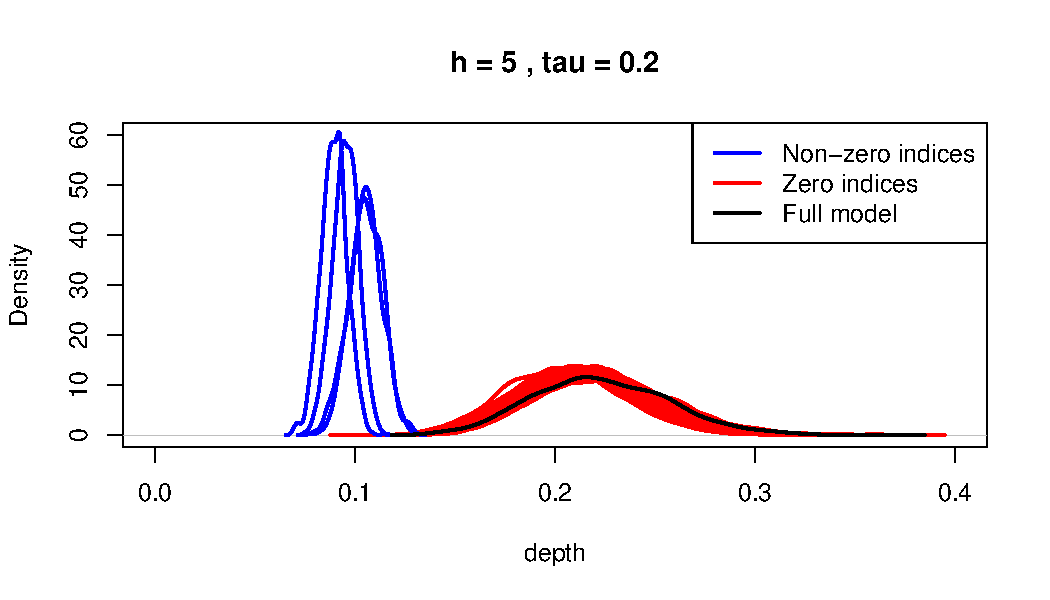
\includegraphics[height=.22\textheight]{../Codes/plot_h5_tau2}\\
%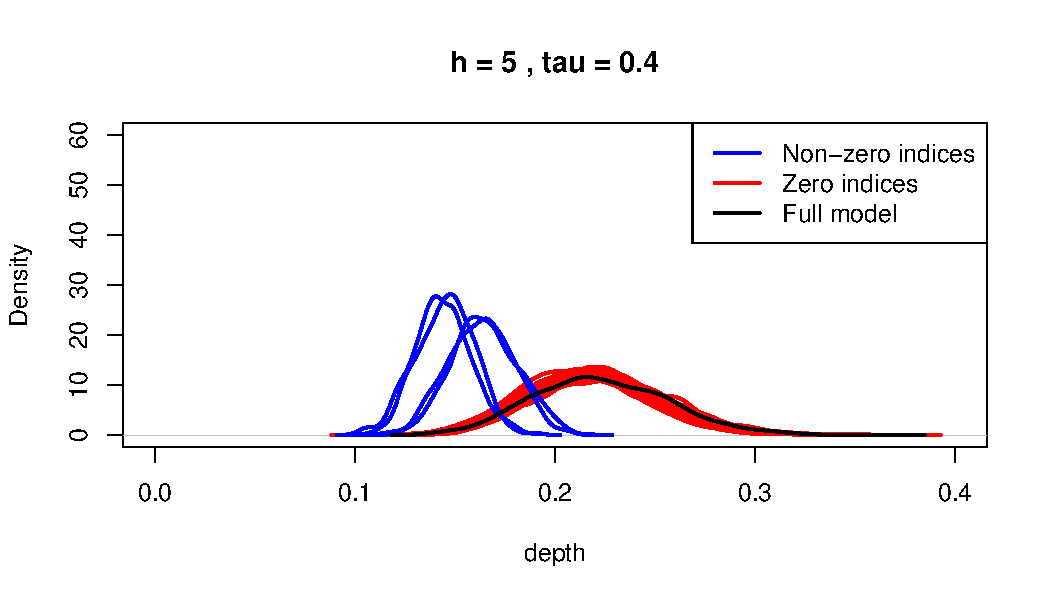
\includegraphics[height=.22\textheight]{../Codes/plot_h5_tau4}\\
%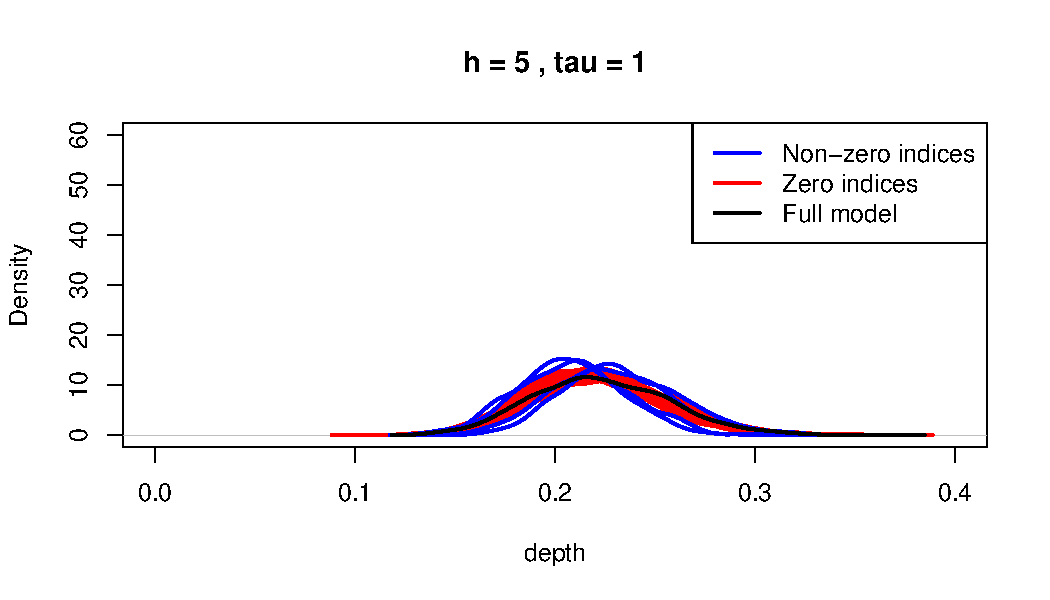
\includegraphics[height=.22\textheight]{../Codes/plot_h5_tau10}\\
%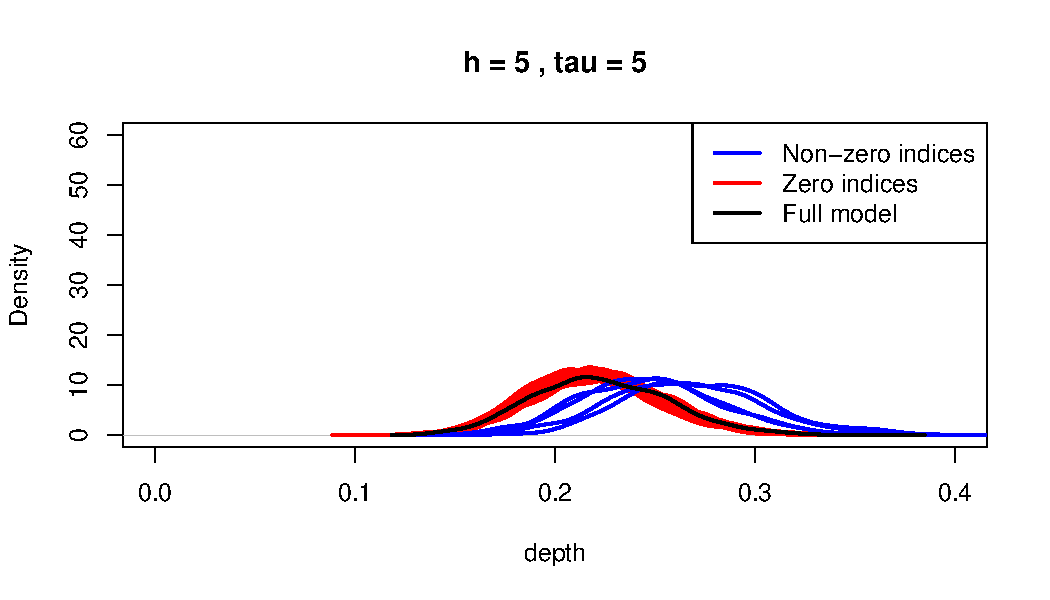
\includegraphics[height=.22\textheight]{../Codes/plot_h5_tau50}
%\caption{Density plots for $\hat \BD(\tau)$ and $\hat \BD_{-j}(\tau)$ for all $j$ in simulation setup, with signal parameter $h=5$ and bootstrap standard deviations $\tau = 0.2, 0.4, 1, 5$}
%\label{fig:figLargeTau1}
%\end{figure}

%\paragraph{(a) Large signal regime ($h=5$: \ref{fig:figLargeTau1})} When $\BD_{-j}$ corresponds to an inadequate model, i.e. the $j$-th coefficient of the true parameter vector is non-zero, for small values of $\tau$ we can clearly distinguish this distribution from that of $\hat\BD (\tau)$ in their density plots. As $\tau$ increases, the inadequate model distributions seem to have more and more positive bias. However, when $j$ is a non-essential covariate, the reduced distributions are close to $\hat \BD(\tau)$ for all values of $\tau$.
%
%\paragraph{(b) Small signal regime ($h=0.05$: \ref{fig:figLargeTau2})} When the actual signal in $\beta_j$ is weak, the inadequate reduced model distributions still approach $\hat \BD(\tau)$ as $\tau$ goes up but stabilize at the full model distribution instead of passing it for very large $\tau$ ($\tau=5$ here). However the adequate model distributions seem to exhibit a similar behavior: albeit staying to the left of inadequate model density plots in general.

%This increased ambiguity of reduced model distributions for small signals make it difficult to distinguish between two types of model distributions using the mean operator, which ends up being very conservative in the second case. For this reason we consider the usage of a different summarizing function that will be able to capture the differentiate between the two types of reduced model distributions across a broader range of the signal-to-noise ratio, specifically by setting a lower detection threshold than the same operator on the full model distribution. Here we focus on a specific alternate formulation of the $e$-value that is based on a tail quantile of $\hat \BD_{-j} (\tau)$:
%%
%\begin{align}
%e_q (\cM_{-j} | \tau) = q \text{-th quantile of } \hat \BD_{-j} (\tau)
%\end{align}
%%
%for some fixed $q \in (0,1)$. Notice that for any $q$, the quantity $e_q (\cM_{-j} | \tau)$ is conditional on the bootstrap standard deviation parameter $\tau$.
%
%The motivation behind this is the observation  
%Also note that we still retain the main flavor of the $e$-values method, by training only the full model and then use Monte Carlo resampling to compute $e_q (\cM_{-j} | \tau)$ for all $j$ and a range of $\tau$.
\section{Simulation}
\label{sec:SimSection}

We now evaluate the performance of the above formulation of quantile $e$-values in a simulation setup. For this, consider the model in (\ref{eqn:LMMeqn}) with no environmental covariates. We consider familes with MZ twins and first generate the SNP matrices $\bfG_i$. We take a total of $p_g = 50$ SNPs, and to simulate correlation among SNPs in the genome generate them in correlated blocks of 6, 4 ,6, 4 and 30. We set the correlation between two SNPs inside a block at 0.7, and consider the blocks to be uncorrelated. For each parent we generate two independent vectors of length 50 with the above correlation structure, and entries within each block being 0 or 1 following Bernoulli distributions with probabilities 0.2, 0.4, 0.4, 0.25 and 0.25 (Minor Allele Frequency or MAF) for SNPs in the 5 blocks, respectively. The genotype of a person is then determined by taking the sum of these two vectors: thus entries in $\bfG_i$ can take the values 0, 1 or 2. Finally we set the common genotype of the twins by randomly choosing one allele vector from each of the parents and taking their sum.

%We use the R package \texttt{regress} to fit the above model with additive error structure. The package requires specifying the dependency structure of all samples in the data. For ease of representation, we only consider nuclear pedigrees with MZ twins in our simulation study and data analysis, which simplifies the overall relationship matrix $\bfPhi = \text{diag} ( \bfPhi_1, \ldots, \bfPhi_m)$ as $\bfI_m \otimes \bfPhi_{MZ}$. Note that, situations in which the pedigree structure is not nuclear can be readily handled in this situation by supplying the overall $\bfPhi$ matrix. The second overall structural component will be  $\bfI_m \otimes {\bf 1} {\bf 1}^T$.

We repeat the above process for $m=250$ families. In GWAS there are generally a small number of causal SNPs, each explaining small proportions of the overall variability in response variable. To reflect this in our simulation setup, we assume that the first entries in each of the first four blocks above are causal, and each of them explains $h/(\sigma_a^2+\sigma_c^2+\sigma_e^2) \%$ of the overall variability. The term $h$ is known as the \textit{heritability} of the corresponding SNP (and can of course vary across SNPs). The value of the non-zero coefficient in $k$-th group: $k = 1, ..., 4$, say $\beta_k$ is calculated using the formula:
%
\begin{align}
\beta_k = \sqrt{ \frac{h}{(\sigma_a^2+\sigma_c^2+\sigma_e^2). 2 \text{MAF}_k (1 - \text{MAF}_k) }}
\end{align}
%
We fix the following values for the error variance components: $\sigma_a^2 = 4, \sigma_c^2 = 1, \sigma_e^2 = 1$, and generate pedigree-wise response vectors $\bfy_1, \ldots, \bfy_{250}$ using the above setup. To consider different SNP effect sizes, we repeat this setup for $h \in \{10, 7, 5, 3, 2, 1, 0 \}$, generating 1000 datasets for each value of $h$.

\subsection{Methods and metrics}
For this simulated data, we compare our $e$-value based approach using the evaluation maps $E_1$ and $E_2$ in (\ref{eqn:EvaluationExamples}) with two other methods:

{\it (1) Model selection on linear model:} Here we ignore the dependency structure within families by training linear models on the simulated data and selecting SNPs with non-zero effects by backward deletion using a modification of the BIC called mBIC2. This has been showed to give better results than single-marker analysis in GWAS for unrelated individuals \citep{FrommeletEtal12} and provides approximate False Discovery Rate (FDR) control at level 0.05 \citep{BogdanEtal11}.

{\it (2) Single-marker mixed model:} We train single-SNP versions of (\ref{eqn:LMMeqn}) using a fast approximation of the Generalized Least Squares procedure (named Rapid Feasible Generalized Least Squares or RFGLS: \cite{LiEtal11}), obtain marginal $p$-values from corresponding $t$-tests and use the Benjamini-Hochberg (BH) procedure to select significant SNPs at FDR = $0.05$.

With the $e$-value being the $q^\text{th}$ quantile of the evaluation map distribution, we set the detection threshold value at the $t^\text{th}$ multiple of $q$ for some $0 < t < 1$. This means all indices $j$ such that $q^\text{th}$ quantile of the bootstrap approximation of $\BE_{-j} $ is less than the $tq^\text{th}$ quantile of the bootstrap approximation of $\BE_{*}$ will get selected as the set of active predictors. To enforce stricter control on the selected set of SNPs we repeat this for $q \in \{ 0.5, 0.6, 0.7, 0.8, 0.9 \}$, and take the SNPs that get selected for \textit{all} values of $q$ as the final set of selected SNPs.

Finally the above procedure depends on the bootstrap standard deviation parameter $s$. Consequently, we repeat the process for $s  \in \{ 0.3, 0.15, \ldots, 0.95, 2 \}$, and take as the final estimated set of SNPs the SNP set $\hat \cS_t (s)$ that minimizes fixed effect prediction error (PE) on an independently generated test dataset $\{ (\bfy_{test,i}, \bfG_{test,i}), i = 1, \ldots, 250 \}$ from the same setup above:
%
\begin{align*}
& \text{PE}_t (s)  = \sum_{i=1}^{250} \sum_{j=1}^4 \left( y_{test,ij} - \bfg_{test,ij}^T \hat \bfbeta_{\hat \cS_t (s)} \right)^2; \\
& \hat \cS_t = \argmin_s \text{PE}_t (s)
\end{align*}

We use the following metrics to evaluate each method we implement: (1) True Positive (TP), which is the proportion of causal SNPs detected;  (2) True Negative (TN), which is the proportion of non-causal SNPs undetected;  (3) Relaxed True Positive (RTP), which is the: proportion of detecting any SNP in each of the 4 blocks with causal SNPs, i.e. for the selected index set by some method $m$, say $\hat \cS_m$,
%
$$
\text{RTP} ( \hat \cS_m ) = \frac{1}{4} \sum_{i=1}^4 \BI ( \text{Block } i \cap \hat \cS_m \neq \emptyset )
$$
%
and finally (4) Relaxed True Negative (RTN), which is the proportion of SNPs in block 5 undetected. We consider the third and fourth metrics to cover situations in which the causal SNP is not detected itself, but highly correlated SNPs with the causal SNP are. This is common in GWAS \citep{FrommeletEtal12}. Finally, we average all the above proportions over 1000 replications, and repeat the process for two different ranges of $t$ for $E_1$ and $E_2$.

%Although the first two heritability values are larger compared to a typical GWAS setup, we use this setup to demonstrate limitations of the existing methodology even in a vastly simplified setting.

\subsection{Results}
% latex table generated in R 3.3.2 by xtable 1.8-2 package
% Sun Apr 16 18:24:09 2017
% latex table generated in R 3.3.2 by xtable 1.8-2 package
% Sun Apr 16 18:24:48 2017
%\begin{table}
%\begin{footnotesize}
%\centering
%    \begin{tabular}{c|c|c|c|cccc}
%    \hline
%     6x   & mBIC2       & RFGLS  & \multicolumn{5}{|c}{quantile $e$-values}    \\\cline{4-8}
%    Heritability    &           & +BH		 & $q$    & $t=0.8$     & $t=0.7$     & $t=0.6$     & $t=0.5$     \\ \hline
%    ~    & ~         & ~         & 0.9      & 0.95/0.97 & 0.95/0.97 & 0.95/0.98 & 0.94/0.98 \\
%    $h=10$ & 0.79/0.99 & 0.95/0.92 & 0.5      & 0.96/0.97 & 0.96/0.98 & 0.95/0.98 & 0.94/0.98 \\
%    ~    & ~         & ~         & 0.2      & 0.96/0.94 & 0.96/0.97 & 0.95/0.97 & 0.95/0.98 \\\hline
%    ~    & ~         & ~         & 0.9      & 0.72/0.95 & 0.7/0.96  & 0.69/0.96 & 0.66/0.97 \\
%    $h=5$  & 0.41/0.99 & 0.62/0.97 & 0.5      & 0.78/0.94 & 0.75/0.94 & 0.72/0.95 & 0.71/0.96 \\
%    ~    & ~         & ~         & 0.2      & 0.83/0.91 & 0.78/0.94 & 0.75/0.95 & 0.73/0.95 \\\hline
%    ~    & ~         & ~         & 0.9      & 0.26/0.97 & 0.24/0.97 & 0.23/0.98 & 0.21/0.98 \\
%    $h=2$  & 0.11/0.99 & 0.14/0.99 & 0.5      & 0.34/0.95 & 0.28/0.96 & 0.27/0.97 & 0.26/0.97 \\
%    ~    & ~         & ~         & 0.2      & 0.46/0.91 & 0.34/0.95 & 0.3/0.96  & 0.27/0.96 \\\hline
%    ~    & ~         & ~         & 0.9      & 0.12/0.98 & 0.1/0.98  & 0.09/0.99 & 0.08/0.99 \\
%    $h=1$  & 0.05/0.99 & 0.04/0.99    & 0.5      & 0.16/0.96 & 0.13/0.97 & 0.12/0.97 & 0.11/0.98 \\
%    ~    & ~         & ~         & 0.2      & 0.25/0.93 & 0.16/0.96 & 0.13/0.97 & 0.13/0.97 \\\hline
%    ~    & ~         & ~         & 0.9      & --/0.99 & --/0.99 & --/0.99 & --/0.99    \\
%    $h=0$  & --/0.99 & --/0.99       & 0.5      & --/0.98 & --/0.98 & --/0.99 & --/0.99 \\
%    ~    & ~         & ~         & 0.2      & --/0.94 & --/0.98 & --/0.98 & --/0.99 \\\hline
%    \end{tabular}
%    \caption{Average True Positive (TP) and True Negative (TN) proportions over 1000 replications for all three methods}
%    \label{table:SNPSimTable0}
%\end{footnotesize}
%\end{table}

%% latex table generated in R 3.3.2 by xtable 1.8-2 package
%% Sun Apr 16 18:24:09 2017
%% latex table generated in R 3.3.2 by xtable 1.8-2 package
%% Sun Apr 16 18:24:48 2017
%\begin{table}
%\begin{footnotesize}
%\centering
%    \begin{tabular}{c|c|c|c|cccc}
%    \hline
%    6x    & mBIC2       & RFGLS  & \multicolumn{5}{|c}{quantile $e$-values}    \\\cline{4-8}
%    Heritability    &           & +BH		 & $q$    & $t=0.8$     & $t=0.7$     & $t=0.6$     & $t=0.5$     \\ \hline
%     ~    & 0.27/0.98 & 0.96/0.99 & 0.9      & 0.95/0.97 & 0.95/0.97 & 0.94/0.97 & 0.94/0.98 \\
%    ~    & ~         & ~         & 0.5      & 0.98/0.96 & 0.97/0.97 & 0.96/0.97 & 0.96/0.97 \\
%    h=10 & ~         & ~         & 0.2      & 0.99/0.9  & 0.97/0.96 & 0.97/0.97 & 0.96/0.97 \\
%    ~    & ~         & ~         & 0.1      & 0.99/0.83 & 0.98/0.93 & 0.97/0.96 & 0.96/0.97 \\
%    ~    & ~         & ~         & 0.05     & 0.99/0.74 & 0.98/0.88 & 0.97/0.94 & 0.97/0.96 \\ \hline
%    ~    & 0.16/0.98 & 0.63/0.99 & 0.9      & 0.74/0.95 & 0.73/0.95 & 0.71/0.96 & 0.69/0.97 \\
%    ~    & ~         & ~         & 0.5      & 0.83/0.93 & 0.78/0.94 & 0.76/0.95 & 0.75/0.95 \\
%    h=5  & ~         & ~         & 0.2      & 0.9/0.87  & 0.83/0.93 & 0.79/0.94 & 0.76/0.95 \\
%    ~    & ~         & ~         & 0.1      & 0.93/0.79 & 0.86/0.9  & 0.81/0.93 & 0.78/0.94 \\
%    ~    & ~         & ~         & 0.05     & 0.95/0.72 & 0.88/0.86 & 0.83/0.91 & 0.79/0.93 \\ \hline
%    ~    & 0.09/0.98 & 0.16/1    & 0.9      & 0.32/0.96 & 0.29/0.97 & 0.27/0.97 & 0.24/0.98 \\
%    ~    & ~         & ~         & 0.5      & 0.45/0.94 & 0.34/0.96 & 0.32/0.96 & 0.3/0.97  \\
%    h=2  & ~         & ~         & 0.2      & 0.66/0.86 & 0.47/0.93 & 0.38/0.95 & 0.33/0.96 \\
%    ~    & ~         & ~         & 0.1      & 0.77/0.79 & 0.57/0.9  & 0.43/0.94 & 0.37/0.95 \\
%    ~    & ~         & ~         & 0.05     & 0.82/0.71 & 0.64/0.85 & 0.5/0.92  & 0.41/0.94 \\ \hline
%    ~    & 0.07/0.98 & 0.05/1    & 0.9      & 0.16/0.97 & 0.14/0.98 & 0.13/0.98 & 0.11/0.99 \\
%    ~    & ~         & ~         & 0.5      & 0.26/0.95 & 0.18/0.97 & 0.17/0.97 & 0.15/0.98 \\
%    h=1  & ~         & ~         & 0.2      & 0.5/0.88  & 0.28/0.94 & 0.2/0.96  & 0.17/0.97 \\
%    ~    & ~         & ~         & 0.1      & 0.65/0.79 & 0.4/0.91  & 0.26/0.95 & 0.2/0.97  \\
%    ~    & ~         & ~         & 0.05     & 0.73/0.71 & 0.51/0.86 & 0.35/0.92 & 0.24/0.95 \\ \hline
%    ~    & 0.05/0.98 & 0.01/1    & 0.9      & 0.04/0.98 & 0.04/0.99 & 0.03/0.99 & 0.03/0.99 \\
%    ~    & ~         & ~         & 0.5      & 0.1/0.97  & 0.05/0.98 & 0.04/0.98 & 0.04/0.98 \\
%    h=0  & ~         & ~         & 0.2      & 0.32/0.89 & 0.1/0.96  & 0.06/0.98 & 0.05/0.98 \\
%    ~    & ~         & ~         & 0.1      & 0.5/0.82  & 0.22/0.93 & 0.1/0.97  & 0.06/0.98 \\
%    ~    & ~         & ~         & 0.05     & 0.64/0.73 & 0.37/0.87 & 0.2/0.94  & 0.09/0.97 \\ \hline
%    \end{tabular}
%    \caption{Average Relaxed True Positive (RTP) and Relaxed True Negative (RTN) proportions over 1000 replications for all three methods}
%    \label{table:SNPSimTable1}
%\end{footnotesize}
%\end{table}
%\begin{table}
%\begin{footnotesize}
%\centering
%    \begin{tabular}{c|c|c|c|cccc}
%    \hline
%    6x    & mBIC2       & RFGLS  & \multicolumn{5}{|c}{quantile $e$-values}    \\\cline{4-8}
%    Heritability    &           & +BH		 & $q$    & $t=0.8$     & $t=0.7$     & $t=0.6$     & $t=0.5$     \\ \hline
%    ~    & ~         & ~         & 0.9      & 0.96/0.97 & 0.96/0.97 & 0.95/0.98 & 0.94/0.98 \\
%    $h=10$ & 0.84/0.99 & 0.96/0.99 & 0.5      & 0.96/0.97 & 0.96/0.97 & 0.95/0.98 & 0.95/0.98 \\
%    ~    & ~         & ~         & 0.2      & 0.97/0.95 & 0.96/0.97 & 0.96/0.97 & 0.95/0.98 \\\hline
%    ~    & ~         & ~         & 0.9      & 0.73/0.95 & 0.71/0.95 & 0.7/0.96  & 0.67/0.97 \\
%    $h=5$  & 0.48/0.99 & 0.64/0.99 & 0.5      & 0.79/0.93 & 0.76/0.94 & 0.73/0.95 & 0.72/0.95 \\
%    ~    & ~         & ~         & 0.2      & 0.85/0.91 & 0.79/0.93 & 0.76/0.94 & 0.74/0.95 \\\hline
%    ~    & ~         & ~         & 0.9      & 0.29/0.96 & 0.27/0.97 & 0.25/0.98 & 0.23/0.98 \\
%    $h=2$  & 0.16/0.99 & 0.16/0.99    & 0.5      & 0.37/0.95 & 0.31/0.96 & 0.3/0.96  & 0.29/0.97 \\
%    ~    & ~         & ~         & 0.2      & 0.53/0.91 & 0.38/0.95 & 0.33/0.95 & 0.3/0.96  \\\hline
%    ~    & ~         & ~         & 0.9      & 0.15/0.97 & 0.13/0.98 & 0.12/0.98 & 0.1/0.99  \\
%    $h=1$  & 0.08/0.99 & 0.05/0.99    & 0.5      & 0.2/0.96  & 0.17/0.97 & 0.15/0.97 & 0.13/0.98 \\
%    ~    & ~         & ~         & 0.2      & 0.35/0.93 & 0.21/0.96 & 0.17/0.97 & 0.16/0.97 \\\hline
%    ~    & ~         & ~         & 0.9      & --/0.97 & --/0.98 & --/0.98 & --/0.99 \\
%    $h=0$  & --/0.98 & --/0.99    & 0.5      & --/0.95 & --/0.97 & --/0.97 & --/0.98 \\
%    ~    & ~         & ~         & 0.2      & --/0.90 & --/0.95 & --/0.97 & --/0.97 \\\hline
%    \end{tabular}
%    \caption{Average Relaxed True Positive (RTP) and Relaxed True Negative (RTN) proportions over 1000 replications for all three methods}
%    \label{table:SNPSimTable1}
%\end{footnotesize}
%\end{table}

% latex table generated in R 3.3.2 by xtable 1.8-2 package
% Mon May 29 17:52:12 2017
%\begin{table}[t]
%\begin{footnotesize}
%\centering
%\begin{tabular}{c|c|c|ccccc}
%  \hline
%  & mBIC2 & RFGLS+BH & $t=\exp(-1)$ & $t=\exp(-2)$ & $t=\exp(-3)$ & $t=\exp(-4)$ & $t=\exp(5)$ \\ 
%  \hline
%$h=10$ & 0.79/0.99 & 0.95/0.92 & 0.95/0.98 & 0.94/0.98 & 0.94/0.99 & 0.92/0.99 & 0.9/0.99 \\ 
%  $h=7$ & 0.59/0.99 & 0.82/0.95 & 0.87/0.97 & 0.85/0.98 & 0.82/0.98 & 0.79/0.99 & 0.75/0.99 \\ 
%  $h=5$ & 0.41/0.99 & 0.62/0.97 & 0.74/0.97 & 0.69/0.98 & 0.65/0.98 & 0.61/0.99 & 0.55/0.99 \\ 
%  $h=3$ & 0.2/0.99 & 0.29/0.98 & 0.47/0.97 & 0.43/0.98 & 0.37/0.99 & 0.32/0.99 & 0.26/1 \\ 
%  $h=2$ & 0.11/0.99 & 0.14/0.99 & 0.28/0.97 & 0.25/0.98 & 0.2/0.99 & 0.17/0.99 & 0.13/1 \\ 
%  $h=1$ & 0.05/0.99 & 0.04/1 & 0.12/0.98 & 0.09/0.99 & 0.07/0.99 & 0.06/1 & 0.04/1 \\ 
%  $h=0$ & 0.01/0.99 & 0/1 & 0.01/0.99 & 0.01/0.99 & 0/1 & 0/1 & 0/1 \\ 
%   \hline
%\end{tabular}
%\caption{Average True Positive (TP) and True Negative (TN) proportions over 1000 replications for all three methods and $E_1$}
%\label{table:SNPSimTable0}
%\end{footnotesize}
%\end{table}
%
%% latex table generated in R 3.3.2 by xtable 1.8-2 package
%% Mon May 29 17:53:11 2017
%\begin{table}[t]
%\begin{footnotesize}
%\centering
%\begin{tabular}{c|c|c|ccccc}
%  \hline
%  & mBIC2 & RFGLS+BH & $t=\exp(-1)$ & $t=\exp(-2)$ & $t=\exp(-3)$ & $t=\exp(-4)$ & $t=\exp(5)$ \\ 
%  \hline
%  $h=10$ & 0.84/0.99 & 0.96/0.99 & 0.95/0.98 & 0.94/0.99 & 0.94/0.99 & 0.92/0.99 & 0.9/0.99 \\ 
%  $h=7$ & 0.66/0.99 & 0.83/0.99 & 0.87/0.97 & 0.85/0.98 & 0.83/0.99 & 0.8/0.99 & 0.75/0.99 \\ 
%  $h=5$ & 0.48/0.99 & 0.64/0.99 & 0.75/0.97 & 0.71/0.98 & 0.67/0.99 & 0.62/0.99 & 0.56/0.99 \\ 
%  $h=3$ & 0.26/0.99 & 0.32/0.99 & 0.5/0.97 & 0.45/0.98 & 0.39/0.99 & 0.33/0.99 & 0.27/1 \\ 
%  $h=2$ & 0.16/0.99 & 0.16/1 & 0.32/0.98 & 0.28/0.98 & 0.22/0.99 & 0.18/0.99 & 0.14/1 \\ 
%  $h=1$ & 0.08/0.99 & 0.05/1 & 0.15/0.98 & 0.12/0.99 & 0.09/0.99 & 0.07/1 & 0.05/1 \\ 
%  $h=0$ & 0.03/0.99 & 0.01/1 & 0.04/0.99 & 0.03/0.99 & 0.02/1 & 0.01/1 & 0.01/1 \\ 
%   \hline
%\end{tabular}
%\caption{Average Relaxed True Positive (RTP) and Relaxed True Negative (RTN) proportions over 1000 replications for all three methods and $E_1$}
%\label{table:SNPSimTable1}
%\end{footnotesize}
%\end{table}
\begin{table}[b]
\centering
\begin{scriptsize}
    \begin{tabular}{c|l|lllllll}
    \hline
    \multicolumn{2}{c|}{Method}          & $h = 10$    & $h = 7$     & $h = 5$     & $h = 3$     & $h = 2$     & $h = 1$     & $h = 0$     \\ \hline
    \multicolumn{2}{c|}{mBIC2}           & 0.79/0.99 & 0.59/0.99 & 0.41/0.99 & 0.2/0.99  & 0.11/0.99 & 0.05/0.99 & -/0.99 \\
    \multicolumn{2}{c|}{RFGLS+BH}        & 0.95/0.92 & 0.82/0.95 & 0.62/0.97 & 0.29/0.98 & 0.14/0.99 & 0.04/1    & -/1       \\ \hline
    ~        & $t = \exp(-1)$ & 0.95/0.98 & 0.87/0.97 & 0.74/0.97 & 0.47/0.97 & 0.28/0.97 & 0.12/0.98 & -/0.99 \\
    ~        & $t = \exp(-2)$ & 0.94/0.98 & 0.85/0.98 & 0.69/0.98 & 0.43/0.98 & 0.25/0.98 & 0.09/0.99 & -/0.99 \\
    $E_1$    & $t = \exp(-3)$ & 0.94/0.99 & 0.82/0.98 & 0.65/0.98 & 0.37/0.99 & 0.2/0.99  & 0.07/0.99 & -/1       \\
    ~        & $t = \exp(-4)$ & 0.92/0.99 & 0.79/0.99 & 0.61/0.99 & 0.32/0.99 & 0.17/0.99 & 0.06/1    & -/1       \\
    ~        & $t = \exp(-5)$ & 0.9/0.99  & 0.75/0.99 & 0.55/0.99 & 0.26/1    & 0.13/1    & 0.04/1    & -/1       \\ \hline
    ~        & $t = 0.8$    & 0.97/0.98 & 0.9/0.97  & 0.79/0.96 & 0.54/0.96 & 0.34/0.97 & 0.15/0.98 & -/0.99 \\
    ~        & $t = 0.74$   & 0.96/0.98 & 0.88/0.97 & 0.75/0.97 & 0.48/0.97 & 0.29/0.98 & 0.12/0.98 & -/0.99 \\
    $E_2$    & $t = 0.68$   & 0.95/0.99 & 0.87/0.98 & 0.72/0.98 & 0.45/0.98 & 0.26/0.98 & 0.1/0.99  & -/0.99 \\
    ~        & $t = 0.62$   & 0.95/0.99 & 0.84/0.98 & 0.68/0.98 & 0.4/0.99  & 0.22/0.99 & 0.09/0.99 & -/0.99    \\
    ~        & $t = 0.56$   & 0.94/0.99 & 0.82/0.99 & 0.65/0.99 & 0.36/0.99 & 0.19/0.99 & 0.07/1    & -/1       \\
    ~        & $t = 0.5$    & 0.92/0.99 & 0.79/0.99 & 0.6/0.99  & 0.31/0.99 & 0.16/1    & 0.05/1    & -/1       \\ \hline
    \end{tabular}
    
\vspace{1em}

        \begin{tabular}{c|l|lllllll}
    \hline
    \multicolumn{2}{c|}{Method}          & $h = 10$    & $h = 7$     & $h = 5$     & $h = 3$     & $h = 2$     & $h = 1$     & $h = 0$     \\ \hline
    \multicolumn{2}{c|}{mBIC2}           & 0.84/0.99 & 0.66/0.99 & 0.48/0.99 & 0.26/0.99 & 0.16/0.99 & 0.08/0.99 & -/0.98 \\
    \multicolumn{2}{c|}{RFGLS+BH}        & 0.96/0.99 & 0.83/0.99 & 0.64/0.99 & 0.32/0.99 & 0.16/1    & 0.05/1    & -/1    \\ \hline
    ~        & $t = \exp(-1)$ & 0.95/0.98 & 0.87/0.97 & 0.75/0.97 & 0.5/0.97  & 0.32/0.98 & 0.15/0.98 & -/0.98 \\
    ~        & $t = \exp(-2)$ & 0.94/0.99 & 0.85/0.98 & 0.71/0.98 & 0.45/0.98 & 0.28/0.98 & 0.12/0.99 & -/0.98 \\
    $E_1$    & $t = \exp(-3)$ & 0.94/0.99 & 0.83/0.99 & 0.67/0.99 & 0.39/0.99 & 0.22/0.99 & 0.09/0.99 & -/0.99    \\
    ~        & $t = \exp(-4)$ & 0.92/0.99 & 0.8/0.99  & 0.62/0.99 & 0.33/0.99 & 0.18/0.99 & 0.07/1    & -/1    \\
    ~        & $t = \exp(-5)$ & 0.9/0.99  & 0.75/0.99 & 0.56/0.99 & 0.27/1    & 0.14/1    & 0.05/1    & -/1    \\ \hline
    ~        & $t = 0.8$    & 0.97/0.98 & 0.91/0.97 & 0.8/0.96  & 0.57/0.96 & 0.38/0.97 & 0.2/0.98  & -/0.97 \\
    ~        & $t = 0.74$   & 0.96/0.98 & 0.89/0.98 & 0.76/0.97 & 0.51/0.97 & 0.33/0.98 & 0.15/0.98 & -/0.98 \\
    $E_2$    & $t = 0.68$   & 0.95/0.99 & 0.87/0.98 & 0.73/0.98 & 0.48/0.98 & 0.29/0.98 & 0.12/0.99 & -/0.98 \\
    ~        & $t = 0.62$   & 0.95/0.99 & 0.85/0.99 & 0.69/0.98 & 0.42/0.99 & 0.24/0.99 & 0.11/0.99 & -/0.99    \\
    ~        & $t = 0.56$   & 0.94/0.99 & 0.83/0.99 & 0.66/0.99 & 0.38/0.99 & 0.2/0.99  & 0.08/0.99 & -/0.99    \\
    ~        & $t = 0.5$    & 0.92/0.99 & 0.79/0.99 & 0.61/0.99 & 0.32/0.99 & 0.17/1    & 0.06/1    & -/1    \\ \hline
    \end{tabular}
\end{scriptsize}
\caption{(Top) Average True Positive (TP), True Negative (TN) and (Bottom) Average Relaxed True Positive (RTP) and Relaxed True Negative (RTN) proportions over 1000 replications for the $e$-values method with $E_1$ and $E_2$ as evaluation maps, and the other two methods}
\label{table:SNPSimTable0}
\end{table}
%


We present the simulation results in table \ref{table:SNPSimTable0}. For all heritability values, applying mBIC2 on linear models performs poorly compared to applying RFGLS and then correcting for multiple testing. This is expected because the linear model ignores the within-family error components.

Our proposed $e$-values work better than the two competing methods for detecting true signals across different values of $h$: the average TP rate going down slowly than other methods across the majority of choices for $t$. Both mBIC2 and RFGLS+BH have very high true negative detection rates, which is matched by our method for higher values of $q$. Since all reduced model distributions reside on the left of the full model distribution, we expect the variable selection process to turn more conservative at lower values of $t$.This effect is more noticeable for lower $q$. This indicates that the right tails of evaluation map distributions are more useful for this purpose. Finally for $h=0$, we report only TN and RTN values since no signals should ideally be detected: in terms of this a value of $q=0.9$ or $q=0.5$ leads to the same TN and RTN performance as RFGLS+BH for all choices of $t$.

RTP performances for all methods are better than the corresponding TP/TN performances. However, for mBIC2 this seems to be due to detecting SNPs in the first four blocks by chance since for $h=0$ its RTN is less than TN. Also $E_2$ seems to perform slightly better than $E_1$, in the sense that it yields a higher TP (or RTP) while having the same TN (or RTN) rates.

%Considering that when analyzing a large number of SNPs false positives need to be minimized, setting $q=0.9, t=0.5$ is a safe choice choice for $e$-values in this simulation setup. Note here that the previous model selection algorithm using $e$-values depended on comparing the mean of the evaluation map distribution $\BE_{-j,n}$ with that of $\BE_{* n}$. Compared to that here we end up comparing a tail quantile of $\BE_{-j,n}$, and set the detection threshold at a smaller value than the same quantile of $\BE_{* n}$.
\section{Analysis of the MCTFR data}
\label{sec:DataSection}

We now apply the above methods on SNPs from the MCTFR dataset. We assume a nuclear pedigree structure, and for simplicity only analyze pedigrees with MZ and DZ twins. After setting aside samples with missing response variables, we end up with 1019 such 4-member families. We look at the effect of genetic factors behind the response variable pertaining to the amount of alcohol consumption, which is highly heritable in this dataset according to previous studies \citep{McGueEtal13}. We analyze SNPs inside some of the most-studied genes with respect to alcohol abuse: GABRA2, ADH1A, ADH1B, ADH1C, ADH4-ADH7, SLC6A3, SLC6A4, OPRM1, CYP2E1, DRD2, ALDH2, and COMT \citep{CoombesThesis16} through separate gene-level models. Any of the ADH genes did not contain many SNPs individually, so we consider the SNPs in all seven of them together. We include sex, birth year, age and generation (parent or offspring) of individuals as covariates to control for their potential effect.

For model selection we use $E_2$ as the evaluation function because of its slighty better performance in the simulations. For each gene-level model, We train the LMM in (\ref{eqn:LMMeqn}) on 75\% of randomly selected families, perform our $e$-values procedure for $s = 0.2, 0.4, \ldots, 2.8, 3, t = 0.1, 0.15, \ldots, 0.75, 0.8$; and select the set of SNPs that minimizes fixed effect prediction error on the data from the other 25\% of families over this grid of $(s,t)$.  

\begin{table}
    \begin{tabular}{l|l|lll}
    \hline
    Gene   & Total no. & \multicolumn{3}{l}{No. of SNPs detected by }\\\cline{3-5}
    & of SNPs & $e$-value & RFGLS+BH & mBIC2 \\\hline
    GABRA2 & 11        & 5       & 0     & 0     \\
    ADH    & 44        & 3       & 1     & 0     \\
    OPRM1  & 47        & 25      & 1     & 0     \\
    CYP2E1 & 9         & 5       & 0     & 0     \\
    ALDH2  & 6         & 5       & 0     & 1     \\
    COMT   & 15        & 14      & 0     & 0     \\
    SLC6A3 & 18        & 4       & 0     & 0     \\
    SLC6A4 & 5         & 0       & 0     & 0     \\
    DRD2   & 17        & 0       & 0     & 1     \\\hline
    \end{tabular}
    \caption{Table of analyzed genes and number of detected SNPs in them by the three methods}
    \label{table:genetable}
\end{table}

As seen in Table~\ref{table:genetable}, our $e$-value based technique detects a much higher number of SNPs than the two competing methods. Our method selects all but one SNP in the genes ALDH2 and COMT. These are small genes of size 50kb and 30kb, respectively, thus SNPs within them have more chance of being in high Linkage Disequilibrium (LD). On the other hand, it does not select any SNPs in SLC6A4 and DRD2. Variants of these genes are known to interact with each other and are jointly associated with multiple behavioral disorders \citep{KarpyakEtal10, WangEtal14}.

\begin{table}
    \begin{tabular}{l|p{2in}|p{1.5in}}
    \hline
    Gene      & Detected SNPs with                              & Reference for \\
    & known associations & associated SNP                              \\\hline
    GABRA2    & rs1808851, rs279856: close to rs279858                         & \cite{CuiEtal12}                                                    \\\hline
    ADH genes & rs17027523: 20kb upstream of rs1229984 & Multiple studies (\url{https://www.snpedia.com/index.php/Rs1229984}) \\\hline
    OPRM1     & rs12662873: 1 kb upstream of rs1799971                            & Multiple studies (\url{https://www.snpedia.com/index.php/Rs1799971}) \\\hline
    CYP2E1    & rs9419624: 600b downstream of rs4646976; rs9419702: 10kb upstream of rs4838767 & \cite{LindEtal12}\\\hline
    ALDH2     & rs16941437: 10kb upstream of rs671                               & Multiple studies (\url{https://www.snpedia.com/index.php/Rs671}) \\\hline
    COMT      & rs4680, rs165774                                               & \cite{VoiseyEtal11}                                                                               \\\hline
    SLC6A3    & rs464049                                                       & \cite{HuangEtal17}\\\hline
    \end{tabular}
    \caption{Table of detected SNPs with known references}
    \label{table:genetable2}
\end{table}

A number of SNPs we detect (or SNPs situated close to them) have known associations with alcohol-related behavioral disorders. We summarize this in Table~\ref{table:genetable2}. Prominent among them are rs1808851 and rs279856 in the GABRA2 gene, which are at perfect LD with rs279858 in the larger, 7188-individual version of our twin studies dataset \citep{IronsThesis12}. This SNP is the marker in GABRA2 that is most frequently associated in the literature with alcohol abuse \citep{CuiEtal12}, but was not genotyped in our sample. A single SNP RFGLS analysis of the same twin studies data that used Bonferroni correction on marginal $p$-values missed the SNPs we detect \citep{IronsThesis12}: highlighting the advantage of our approach. We give a gene-wise discussion of associated SNPs, as well as information on all SNPs, in the supplementary material.

\begin{figure}
\begin{center}

\begin{tabular}{c}
		\includegraphics[height=.4\textwidth]{{"plotMZDZ_GABRA2"}.png}\\
		(a)\\
		\includegraphics[height=.4\textwidth]{{"plotMZDZ_ADH"}.png} \\
		(b)\\	
		\includegraphics[height=.4\textwidth]{{"plotMZDZ_OPRM1"}.png}\\
		(c)\\	
\end{tabular}

\caption{Plot of $e$-values for genes analyzed: (a) GABRA2, (b) ADH1 to ADH7, (c) OPRM1. For ease of visualization, $1 - e$-values are plotted in the y-axis.}
\label{fig:geneplot1}

\end{center}
\end{figure}

\begin{figure}
\begin{center}

\begin{tabular}{c}
		\includegraphics[height=.4\textwidth]{{"plotMZDZ_CYP2E1"}.png}\\
		(d)\\
		\includegraphics[height=.4\textwidth]{{"plotMZDZ_ALDH2"}.png} \\
		(e)\\	
		\includegraphics[height=.4\textwidth]{{"plotMZDZ_COMT"}.png}\\
		(f)\\	
\end{tabular}

\caption{Plot of $e$-values for genes analyzed: (d) CYP2E1, (e) ALDH2, (f) COMT}
\label{fig:geneplot2}

\end{center}
\end{figure}

\begin{figure}
\begin{center}

\begin{tabular}{c}
		\includegraphics[height=.4\textwidth]{{"plotMZDZ_SLC6A3"}.png}\\
		(g)\\
		\includegraphics[height=.4\textwidth]{{"plotMZDZ_SLC6A4"}.png} \\
		(h)\\	
		\includegraphics[height=.4\textwidth]{{"plotMZDZ_DRD2"}.png}\\
		(i)\\	
\end{tabular}

\caption{Plot of $e$-values for genes analyzed: (g) SLC6A3, (h) SLC6A4, (i) DRD2}
\label{fig:geneplot3}

\end{center}
\end{figure}

We plot the $90^{\Th}$ quantile $e$-value estimates in Figures~\ref{fig:geneplot1}, \ref{fig:geneplot2} and \ref{fig:geneplot3}. We obtained gene locations, as well as the locations of coding regions of genes, i.e. exons, inside 6 of these 9 genes from annotation data extracted from the UCSC Genome Browser database \citep{UCSCdata}. Exon locations were not available for OPRM1, CYP2E1 and DRD2. In general, SNPs tend to get selected in groups with neighboring SNPs, which suggests high LD. Also most of the selected SNPs either overlap or in close proximity to the exons, which underline their functional relevance.
\section{Discussion and conclusion}
\label{sec:endSection}

%In the above sections we have proposed a fast covariate selection method to detect SNP signals in multi-SNP mixed effect models. The speed advantage is achieved because of two reasons: calculation of only a single model for the full algorithm, and utilizing a parallelizable bootstrap technique that uses only Monte-Carlo samples and previously obtained model objects to get resampling estimates of the coefficient vector. Our method achieves this by using the recently proposed $e$-values framework and comparing sampling distributions of reduced model estimates with that of the full model through an evaluation map function.

To expand the above approach to a genome-wide scale, we need to incorporate strategies for dealing with the hierarchical structure of causal SNPs: there are a few causal genes behind a quantitative phenotype, which can be further attributed to a proportion of SNPs inside each gene. To apply the $e$-values method here, it is plausible to start with an initial screening step to eliminate evidently non-relevant genes. Methods like the grouped Sure Independent Screening \citep{LiZhongZhu12} and min-P test \citep{WestfallYoungBook93} can be useful here. Following this, in a multi-gene predictor set, there are several possible strategies to select important genes \textit{and} important SNPs in them. Firstly, one can use a two-stage $e$-value based procedure. The first stage is same as the method described in this paper, i.e. selecting important SNPs from each gene using multi-SNP models trained on SNPs in that gene. In the second stage, a model will be trained using the aggregated set of SNPs obtained in the first step, and a group selection procedure will be run on this model using $e$-values. This means dropping \textit{groups} of predictors (instead of single predictors) from the full model, checking the reduced model $e$-values, and selecting a SNP group only if dropping it causes the $e$-value to go below a certain cutoff. Secondly, one can start by selecting important genes using an aggregation method of SNP-trait associations (e.g. \cite{LamparterEtal16}) and then run the $e$-value based SNP selection on the set of SNPs within these genes. Thirdly, one can also take the aggregated set of SNPs obtained from running the $e$-values procedure on gene-level models, then use a fast screening method (e.g. RFGLS) to select a subset of those SNPs.

We plan to study merits and demerits of these strategies and the computational issues associated with them in detail through synthetic studies as well as in the GWAS data from MCTFR. Finally, the current evaluation map based formulation requires the existence of an asymptotic distribution for the full model estimate. We plan to explore alternative formulation of evaluation maps under weaker conditions to bypass this, so as to be able to tackle high-dimensional ($n < p$) situations.

%\section*{Acknowledgements}
%SM acknowledges the University of Minnesota Interdisciplinary Doctoral Fellowship program.
%SC is partially supported by the National Science Foundation (NSF) under grants \# DMS-1622483, \# DMS-1737918.

\bibliographystyle{apalike}
%\bibliographystyle{imsart-number}
%\bibliography{snpbib}
\bibliography{Twin-studies-e-values}

\documentclass[fleqn,12pt]{article}

\usepackage{mycommands,amssymb,amsmath,amsthm,color,pagesize,outlines,cite,subfigure}
\usepackage[small]{caption}
\usepackage[pdftex]{epsfig}
\usepackage{hyperref} % for linking references 
\usepackage{stackrel}
\usepackage{rotating} % sideways table

\usepackage[round]{natbib}

% for algorithm
\usepackage[noend]{algpseudocode}
\usepackage{algorithm}

%% measurements for 1 inch margin
\addtolength{\oddsidemargin}{-.875in}
\addtolength{\evensidemargin}{-.875in}
\addtolength{\textwidth}{1.75in}
\addtolength{\topmargin}{-.875in}
\addtolength{\textheight}{1.75in}

\usepackage{setspace}
\doublespacing

\usepackage{chngcntr}
\usepackage{apptools}
\AtAppendix{\counterwithin{Theorem}{section}}
\numberwithin{equation}{section}

\begin{document}

\newtheorem{Theorem}{Theorem}[section]
\newtheorem{Lemma}[Theorem]{Lemma}
\newtheorem{Corollary}[Theorem]{Corollary}
\newtheorem{Proposition}[Theorem]{Proposition}
\newtheorem{Conjecture}[Theorem]{Conjecture}
\theoremstyle{definition} \newtheorem{Definition}[Theorem]{Definition}

\title{Supplementary to "Simultaneous Selection of Multiple Important Single Nucleotide Polymorphisms in Familial Genome Wide Association Studies data"}
\date{}
\maketitle

\appendix

\section{Proof of theoretical results}

\begin{proof}[Proof of Theorem 3.2] Define $c_{q,\infty} = q^{\text{th}}$ quantile of $\BT_0$. Now following assumption (E1),
%
\begin{align*}
c_q (\BE_*) &= \inf_\bftheta \{ E(\bftheta, [\hat \bftheta]): \BF_* \geq q \} \\
&= \inf_\bftheta \{ E(a_n(\bftheta - \bftheta_0), [a_n(\hat \bftheta - \bftheta_0)]):  a_n (\BF_* - \bftheta_0) \geq q\}
\end{align*}
%
where $\BF_*$ is the probability distribution function of $E(\hat \bftheta, [\hat \bftheta])$. Part 1 is proved following assumptions (P2) and (E3).

Now if $\cM$ is adequate, following assumption (E1),
%
\begin{align}\label{eqn:Thm1ProofEqn1}
E (\hat \bftheta_m, [\hat \bftheta]) = E( \hat \bftheta	_m - \bftheta_0, [\hat \bftheta - \bftheta_0])
\end{align}
%
Decompose the first argument as
%
\begin{align}\label{eqn:Thm1ProofEqn2}
\hat \bftheta_m - \bftheta &= (\hat \bftheta_m - \hat \bftheta) + (\hat \bftheta - \bftheta_0)
\end{align}
%
By definition, $\hat \theta_{mj} - \hat \theta_j = 0$ if $j \in \cS$, else equals $\theta_{0j} - \hat \theta_j$. Thus for the first summand in (\ref{eqn:Thm1ProofEqn2}) we have
%
$$
\hat \bftheta_m - \hat \bftheta =  O_P (1/a_n)
$$
%
Going back to (\ref{eqn:Thm1ProofEqn1}), this implies
%
$$
| E( \hat \bftheta_m - \bftheta_0, [\hat \bftheta - \bftheta_0]) -
E( \hat \bftheta - \bftheta_0, [\hat \bftheta - \bftheta_0]) | < O_P (a_n^{-\alpha})
$$
%
using lipschitz continuity in assumption (E2), i.e
%
$$
| E( \hat \bftheta_m, [\hat \bftheta]) - E( \hat \bftheta, [\hat \bftheta]) | < O_P (a_n^{-\alpha})
$$
%
again using (E1). Part 2 now follows.

For part 3, we apply (E1) to get
%
\begin{align}\label{eqn:Thm1ProofEqn3}
E (\hat \bftheta_m, [\hat \bftheta]) = E( a_n(\hat \bftheta	_m - \bftheta_0), [a_n(\hat \bftheta - \bftheta_0)])
\end{align}
%
And decompose the first argument as
%
\begin{align}\label{eqn:Thm1ProofEqn4}
a_n(\hat \bftheta_m - \bftheta_0) &= a_n(\hat \bftheta_m - \bftheta_m) + a_n(\bftheta_m - \bftheta_0)
\end{align}
%
Since $\cM$ is inadequate, $\theta_{mj} \neq \theta_{0j}$ when $j \notin \cS$. So $\| a_n(\bftheta_m - \bftheta_0) \| \uparrow \infty$ as $a_n \uparrow \infty$. Applying (E4) now proves part 3.
\end{proof}

\begin{proof}[Proof of Theorem 3.3] The proof is fairly similar to that of theorem 3.2, so we give a sketch of it. For the full model, the bootstrap is consistent, i.e. $a_n (\hat \bftheta_* - \bftheta_0)$ and $(a_n/ \tau_n) (\hat \bftheta_{r*} - \hat \bftheta_*)$ converge to same weak limit in probability, following theorems 2.2 and 2.3 in \cite{MajumdarChatterjee17}. Specifically, conditions (A1)-(A6) in \cite{MajumdarChatterjee17} ensure condition (P2) in our paper through theorem 2.2 therein, following which  theorem 2.3 ensures that when (A1)-(A6) are satisfied, bootstrap consistency holds. The definition of $\hat \bftheta_m$ now means that
$a_n (\hat \bftheta_m - \bftheta_m)$ and $(a_n/ \tau_n) (\hat \bftheta_{rm} - \hat \bftheta_m)$ converge to the same weak limit in probability for any model $\cM$. A similar approach as the proof of parts 2 and 3 of theorem 3.2 now follows, with an additional term corresponding to bootstrap estimates in (\ref{eqn:Thm1ProofEqn2}) and (\ref{eqn:Thm1ProofEqn4}).
\end{proof}

\section{Outputs for MCTFR data analysis}

Each table gives the $90^{\text{th}}$ percentile $e$-values, which are plotted in figures 2, 3, and 4 in main paper, of SNPs analyzed in the gene. Column 'Association' is obtained from the sign of the SNP coefficient in the full model.

% latex table generated in R 3.3.2 by xtable 1.8-2 package
% Fri Oct 13 17:34:26 2017
\begin{table}[ht]
\centering
\begin{tabular}{lccc}
  \hline
SNP name & Location & $e$-value & Association \\ 
  \hline
rs16859227 & 46250605 & 0.89 & + \\ 
  rs572227 & 46251393 & 0.13 & - \\ 
  rs534459 & 46256805 & 0.24 & + \\ 
  rs2119183 & 46272806 & 0.92 & - \\ 
  rs502038 & 46280318 & 0.58 & + \\ 
  rs1808851 & 46311447 & 0.00 & + \\ 
  rs279856 & 46317923 & 0.00 & - \\ 
  rs3775282 & 46321863 & 0.86 & - \\ 
  rs279841 & 46340763 & 0.75 & + \\ 
  rs10805145 & 46358331 & 0.73 & - \\ 
  rs13152740 & 46381221 & 0.86 & - \\ 
   \hline
\end{tabular}
\caption{SNPs for GABRA2, chr4, position 46243548 - 46390039; $e$-value cutoff 0.72}
\end{table}

% latex table generated in R 3.3.2 by xtable 1.8-2 package
% Fri Oct 13 17:34:26 2017
\begin{table}[H]
\centering
\begin{tabular}{lccc}
  \hline
SNP name & Location & $e$-value & Association \\ 
  \hline
rs17027299 & 99078105 & 0.84 & - \\ 
  rs9307222 & 99101051 & 0.76 & - \\ 
  rs10006414 & 99101401 & 0.49 & + \\ 
  rs9994641 & 99101605 & 0.48 & + \\ 
  rs13134014 & 99104879 & 0.75 & - \\ 
  rs6820691 & 99105055 & 0.76 &+\\ 
  rs6820913 & 99125659 & 0.81 &+\\ 
  rs6532729 & 99146436 & 0.67 &-\\ 
  rs13150538 & 99152631 & 0.49 &-\\ 
  rs17027380 & 99157450 & 0.63 &-\\ 
  rs17494998 & 99160699 & 0.41 &+\\ 
  rs549467 & 99172232 & 0.81 &+\\ 
  rs2034677 & 99187874 & 0.62 &+\\ 
  rs12508445 & 99190653 & 0.01 &-\\ 
  rs10003496 & 99197839 & 0.81 &+\\ 
  rs10005811 & 99208603 & 0.02 &+\\ 
  rs603215 & 99214851 & 0.78 &-\\ 
  rs433146 & 99229839 & 0.87 &-\\ 
  rs17027456 & 99235747 & 0.31 &-\\ 
  rs17561798 & 99235941 & 0.85 &+\\ 
  rs10516428 & 99237439 & 0.45 &-\\ 
  rs6532731 & 99251006 & 0.80 &+\\ 
  rs7694221 & 99260423 & 0.90 &+\\ 
  rs10028330 & 99268949 & 0.70 &-\\ 
  rs10022047 & 99296818 & 0.49 &+\\ 
  rs17027523 & 99298979 & 0.05 &+\\ 
  rs17027530 & 99303633 & 0.69 &+\\ 
  rs3775540 & 99304544 & 0.23 &-\\ 
  rs3756088 & 99309404 & 0.89 &-\\ 
  rs13103626 & 99317251 & 0.75 &+\\ 
  rs10516430 & 99337881 & 0.62 &+\\ 
  rs9884594 & 99359318 & 0.68 &-\\ 
  rs12503056 & 99369061 & 0.63 &+\\ 
  rs2004316 & 99381148 & 0.43 &-\\ 
  rs4303985 & 99399748 & 0.87 &-\\ 
  rs4414961 & 99403784 & 0.86 &-\\ 
  rs12509267 & 99407299 & 0.80 &+\\ 
  rs6838913 & 99408106 & 0.84 &-\\ 
  rs4374629 & 99411783 & 0.85 &+\\ 
  rs4527483 & 99421741 & 0.89 &+\\ 
  rs10009693 & 99423280 & 0.90 &-\\ 
  rs10023791 & 99425353 & 0.88 &+\\ 
  rs955931 & 99428163 & 0.88 &-\\ 
  rs17027628 & 99428608 & 0.85 &-\\ 
   \hline
\end{tabular}
\caption{SNPs for ADH genes, chr4, position 99070977 - 99435737; $e$-value cutoff 0.225}
\end{table}

% latex table generated in R 3.3.2 by xtable 1.8-2 package
% Fri Oct 13 17:34:26 2017
\begin{table}[H]
\centering
\begin{tabular}{lccc}
  \hline
SNP name & Location & $e$-value & Association \\ 
  \hline
rs2000371 & 154011024 & 0.39 &-\\ 
  rs9371718 & 154011615 & 0.08 &-\\ 
  rs12211203 & 154016936 & 0.63 &-\\ 
  rs1937600 & 154017197 & 0.02 &-\\ 
  rs9397637 & 154022718 & 0.00 &+\\ 
  rs1937590 & 154036895 & 0.63 &+\\ 
  rs12662873 & 154040810 & 0.18 &+\\ 
  rs12661209 & 154044112 & 0.84 &-\\ 
  rs1316368 & 154055754 & 0.00 &-\\ 
  rs1937587 & 154060023 & 0.27 &-\\ 
  rs6921403 & 154063906 & 0.00 &-\\ 
  rs1937580 & 154076643 & 0.00 &+\\ 
  rs1937645 & 154082228 & 0.00 &+\\ 
  rs1892361 & 154099619 & 0.00 &-\\ 
  rs1937633 & 154104857 & 0.04 &-\\ 
  rs1937631 & 154105011 & 0.00 &-\\ 
  rs12527197 & 154107836 & 0.02 &+\\ 
  rs1892360 & 154111701 & 0.74 &-\\ 
  rs1892359 & 154112042 & 0.65 &-\\ 
  rs1892356 & 154112263 & 0.56 &+\\ 
  rs1937622 & 154113139 & 0.54 &-\\ 
  rs10485258 & 154113409 & 0.72 &-\\ 
  rs1937619 & 154114583 & 0.58 &-\\ 
  rs1748289 & 154121980 & 0.77 &-\\ 
  rs1781619 & 154135968 & 0.64 &-\\ 
  rs652051 & 154139344 & 0.74 &+\\ 
  rs10485262 & 154140199 & 0.69 &-\\ 
  rs9371312 & 154145492 & 0.81 &+\\ 
  rs1332849 & 154151117 & 0.48 &-\\ 
  rs9371749 & 154153369 & 0.28 &+\\ 
  rs9285539 & 154154532 & 0.08 &+\\ 
  rs9322439 & 154156250 & 0.07 &+\\ 
  rs11752884 & 154159710 & 0.25 &-\\ 
  rs4869813 & 154173845 & 0.13 &+\\ 
  rs4870241 & 154174963 & 0.00 &-\\ 
  rs9384156 & 154186720 & 0.13 &+\\ 
  rs2065139 & 154192175 & 0.89 &-\\ 
  rs689219 & 154198820 & 0.00 &-\\ 
  rs9371761 & 154202578 & 0.20 &-\\ 
  rs12199858 & 154204327 & 0.00 &+\\ 
  rs9371762 & 154213973 & 0.00 &-\\ 
  rs612450 & 154214357 & 0.00 &-\\ 
  rs9384159 & 154219177 & 0.00 &+\\ 
  rs6938958 & 154220427 & 0.00 &-\\ 
  rs581564 & 154221214 & 0.00 &+\\ 
  rs12202611 & 154237443 & 0.76 &-\\ 
  rs4870255 & 154237937 & 0.88 &-\\ 
   \hline
\end{tabular}
\caption{SNPs for OPRM1, chr6, position 154010496 - 154246867; $e$-value cutoff 0.225}
\end{table}

% latex table generated in R 3.3.2 by xtable 1.8-2 package
% Fri Oct 13 17:34:26 2017
\begin{table}[ht]
\centering
\begin{tabular}{lccc}
  \hline
SNP name & Location & $e$-value & Association \\ 
  \hline
rs10872828 & 133525348 & 0.72 &-\\ 
  rs9419702 & 133531153 & 0.09 &-\\ 
  rs7083395 & 133532269 & 0.77 &+\\ 
  rs9419624 & 133534822 & 0.06 &+\\ 
  rs7906770 & 133536902 & 0.28 &-\\ 
  rs9419569 & 133541881 & 0.06 &+\\ 
  rs9419629 & 133543210 & 0.06 &+\\ 
  rs7093241 & 133556596 & 0.72 &-\\ 
  rs9419649 & 133561098 & 0.91 &-\\ 
   \hline
\end{tabular}
\caption{SNPs for CYP2E1, chr10, position 133520406 - 133561220; $e$-value cutoff 0.72}
\end{table}

% latex table generated in R 3.3.2 by xtable 1.8-2 package
% Fri Oct 13 17:34:26 2017
\begin{table}[ht]
\centering
\begin{tabular}{lccc}
  \hline
SNP name & Location & $e$-value & Association \\ 
  \hline
rs7398343 & 111774068 & 0.34 &-\\ 
  rs7297186 & 111778178 & 0.36 &+\\ 
  rs3803167 & 111785586 & 0.00 &+\\ 
  rs10219736 & 111788402 & 0.00 &-\\ 
  rs16941437 & 111793039 & 0.00 &-\\ 
  rs3742004 & 111798553 & 0.75 &+\\ 
   \hline
\end{tabular}
\caption{SNPs for ALDH2, chr12, position 111766887 - 111817529; $e$-value cutoff 0.72}
\end{table}

% latex table generated in R 3.3.2 by xtable 1.8-2 package
% Fri Oct 13 17:34:26 2017
\begin{table}[H]
\centering
\begin{tabular}{lccc}
  \hline
SNP name & Location & $e$-value & Association \\ 
  \hline
rs4646312 & 19948337 & 0.41 & -\\ 
  rs165656 & 19948863 & 0.22 & -\\ 
  rs165722 & 19949013 & 0.24 &    +\\ 
  rs2239393 & 19950428 & 0.50 &+\\ 
  rs4680 & 19951271 & 0.60 &+\\ 
  rs4646316 & 19952132 & 0.81 &-\\ 
  rs165774 & 19952561 & 0.72 &-\\ 
  rs174699 & 19954458 & 0.07 &+\\ 
  rs165599 & 19956781 & 0.58 &-\\ 
  rs165728 & 19957023 & 0.02 &-\\ 
  rs165815 & 19959473 & 0.00 &+\\ 
  rs5993891 & 19959746 & 0.04 &-\\ 
  rs887199 & 19961955 & 0.04 &-\\ 
  rs2239395 & 19962203 & 0.07 &+\\ 
  rs2518824 & 19962963 & 0.59 &+\\ 
   \hline
\end{tabular}
\caption{SNPs for COMT, chr22, position 19941607 - 19969975; $e$-value cutoff 0.72}
\end{table}


% latex table generated in R 3.3.2 by xtable 1.8-2 package
% Fri Oct 13 17:34:26 2017
\begin{table}[H]
\centering
\begin{tabular}{lrrr}
  \hline
SNP name & Location & $e$-value & Association \\ 
  \hline
rs27072 & 1394522 & 0.87 &+\\ 
  rs40184 & 1395077 & 0.78 &-\\ 
  rs11564771 & 1398797 & 0.80 &-\\ 
  rs11133767 & 1401580 & 0.79 &+\\ 
  rs6869645 & 1404548 & 0.82 &+\\ 
  rs3776512 & 1407116 & 0.84 &+\\ 
  rs6347 & 1411412 & 0.83 &-\\ 
  rs27048 & 1412645 & 0.90 &-\\ 
  rs2042449 & 1416646 & 0.63 &+\\ 
  rs13161905 & 1417212 & 0.72 &-\\ 
  rs2735917 & 1420268 & 0.92 &+\\ 
  rs464049 & 1423905 & 0.21 &-\\ 
  rs460700 & 1429969 & 0.00 &-\\ 
  rs460000 & 1432825 & 0.00 &+\\ 
  rs4975646 & 1433401 & 0.88 &-\\ 
  rs403636 & 1438354 & 0.78 &-\\ 
  rs2617605 & 1442521 & 0.89 &+\\ 
  rs6350 & 1443199 & 0.93 &+\\ 
   \hline
\end{tabular}
\caption{SNPs for SLC6A3, chr5, position 1392790 - 1445430; $e$-value cutoff 0.72}
\end{table}

% latex table generated in R 3.3.2 by xtable 1.8-2 package
% Fri Oct 13 17:34:26 2017
\begin{table}[H]
\centering
\begin{tabular}{lccc}
  \hline
SNP name & Location & $e$-value & Association \\ 
  \hline
rs16967029 & 30195292 & 0.79 &+\\ 
  rs2051810 & 30195841 & 0.84 &-\\ 
  rs11658318 & 30206059 & 0.72 &-\\ 
  rs8079471 & 30218317 & 0.64 &+\\ 
  rs3760454 & 30222002 & 0.90 &+\\ 
   \hline
\end{tabular}
\caption{SNPs for SLC6A4, chr17, position 30194319 - 30236002; $e$-value cutoff 0.63}
\end{table}

% latex table generated in R 3.3.2 by xtable 1.8-2 package
% Fri Oct 13 17:34:26 2017
\begin{table}[H]
\centering
\begin{tabular}{lccc}
  \hline
SNP name & Location & $e$-value & Association \\ 
  \hline
rs2514229 & 113410000 & 0.87 &-\\ 
  rs11214654 & 113410917 & 0.86 &+\\ 
  rs7937641 & 113415976 & 0.63 &-\\ 
  rs12222458 & 113417603 & 0.73 &-\\ 
  rs10736470 & 113418371 & 0.73 &-\\ 
  rs12576506 & 113419869 & 0.85 &+\\ 
  rs10750025 & 113424042 & 0.66 &+\\ 
  rs7952106 & 113424558 & 0.70 &-\\ 
  rs4373974 & 113430486 & 0.88 &-\\ 
  rs4130345 & 113436487 & 0.88 &-\\ 
  rs7123697 & 113440331 & 0.78 &+\\ 
  rs6589386 & 113443753 & 0.75 &+\\ 
  rs4132966 & 113451589 & 0.86 &+\\ 
  rs7940164 & 113451765 & 0.90 &-\\ 
  rs4245155 & 113457324 & 0.92 &-\\ 
  rs11607834 & 113461680 & 0.92 &-\\ 
  rs12280220 & 113469219 & 0.93 &-\\ 
   \hline
\end{tabular}
\caption{SNPs for DRD2, chr11, position 113409595 - 113475691; $e$-value cutoff 0.63}
\end{table}


\section{Discussion on gene-specific findings in the MCTFR data}
\label{sec:DataSection}

{\it GABRA2:} As seen in the plots, the first two SNPs detected are close to two separate exons. The 4th and 5th detected SNPs, rs1808851 and rs279856, are at perfect LD with rs279858 in the larger 7188-individual dataset \citep{IronsThesis12}. This SNP had not been genotyped in our sample, but is the marker in GABRA2 that is most frequently associated in the literature with alcohol abuse \citep{CuiEtal12}. Interestingly, a single SNP RFGLS analysis of the same twin studies data that used Bonferroni correction on marginal $p$-values to detect SNPs had missed these SNPs \citep{IronsThesis12}. This highlights the advantage of our approach.

{\it ADH genes:} Multiple studies have associated rs1229984 in the ADH1B gene (position 99318162 of chromosome 4) with alcohol dependence (\url{https://www.snpedia.com/index.php/Rs1229984}), which as seen in the plot of ADH2 is close to an exon region. Our data does not contain this marker, but detects one SNP 20 kb upstream of this, rs17027523. Another SNP, rs3775540 at position 99304544 has an $e$-value of 0.226, so narrowly misses detection. This is close to rs1229984, and also rs1042026 at position 99307309, which \cite{MacgregorEtal08} found to be strongly associated with alcohol consumption.

The SNP rs17027523 is interesting: it resides in the uncharacterized long non-coding RNA gene LOC100507053. One previous study \citep{GelernterEtal14, XuEtal15} found significant associations for 5 SNPs in this gene with alcohol consumption for African American population through single-SNP analysis on non-familial GWAS data. Notably, their analysis found a much stronger evidence of the association in African-American part of the sample than the European American part, while our findings are entirely from a Caucasian sample.

{\it OPRM1:} Many of the SNPs analyzed in this gene have very low $e$-values, and tend to cluster together. The minor allele of the SNP rs1799971 (chr 6, position 154039662) has been associated with stronger alcohol cravings (\url{https://www.snpedia.com/index.php/Rs1799971}), and we detect rs12662873 at position 154040810.

{\it CYP2E1:} Five of the 9 SNPs studied are detected through our analysis. Four of them are within 10 kb of one another (base pairs 133534822 to 133543210 in chr 10). In the analysis of \cite{LindEtal12} rs4646976 at 133534223 position was most associated with a measure of breath alcohol concentration: this is within our detected region. This study had also detected rs4838767 in the promoter region of CYP2E1 (position 133520114) associated with multiple alcohol consumption measures. We detect rs9419702 at position 133531153.

{\it ALDH2:} All 6 SNPs we study are close to exons, and 5 get picked up by the $e$-value procedure. While all five are at a lesser base pair position than the well-known SNP rs671 ({\url{https://www.snpedia.com/index.php/Rs671}, position 111803962), one of the SNPs we analyze (rs16941437) is within 10 kb upstream of this SNP.

{\it COMT:} The SNP rs4680 has long been associated with schizophrenia and substance abuse, including alcoholism. A case-control study \citep{VoiseyEtal11} associated rs4680 and rs165774 with alcohol dependence through a SNP-wise chi-squared test, and had these two SNPs in high LD in their study population. Compared to this, in our simultaneous model of all COMT polymorphisms, the more well-known rs4680 has a below threshold $e$-value. 
% A previous case-control GWAS on unrelated individuals with European and African ancestry that also focused on analysis of well-studied genes also did not find any association between rs4680 and alcohol dependence \citep{OlfsonBierut08}.

{\it SLC6A3:} Our analysis does not detect rs27072, which has been associated with alcohol withdrawal symptoms (\url{https://www.snpedia.com/index.php/Rs27072}). 
%
%{\it SLC6A4:} The SNP rs1042173 has repeatedly been associated with alcohol consumption (\url{https://www.snpedia.com/index.php/Rs1042173}). In our analysis, the 3 SNPs closest to this have low $e$-values. One of them has $e$-value lower than the adaptive threshold $t=0.72$, while the other two narrowly miss it.
%
%{\it DRD2:} Five of the 7 SNPs analyzed have lower $e$-values than the rest, and all of them are in a 10 kb region, between positions 113415976 and 113424042 of chromosome 11. Two of these 5 have $e$-values below the gene-specific threshold. This region is within 3 kb upstream of rs1076560, which has multiple references of association with alcoholism (\url{https://www.snpedia.com/index.php/Rs1076560}). All the three DRD2 SNPs associated with alcoholism in a case-control study on an Eastern Indian study sample \citep{BhaskarEtal10}: rs2734835, rs1116313 and TaqID, are either inside or within 5 kb of this region. one of them (rs2734835) is also close to rs7937641, while the other two (rs1116313 and TaqID) are within 4 kb of another detected SNP in our analysis: rs10750025.

Finally, most $e$-values for the last 3 genes, i.e. SLC6A3, SLC6A4 and DRD2, are large: indicating weak SNP signals. We found this observation interesting, because variants of these genes have known interaction effects behind alcohol withdrawal-induced seizure \citep{KarpyakEtal10} and bipolar disorder \citep{WangEtal14}, as well as additive effect on the susceptibility to smoking addiction \citep{ErblichEtal05}.


% For this reason we also ran the $e$-values procedure on the combined set of SNPs from these genes, but did not detect any signal there as well for our sample. %change, look into rs1042173
 
%We detected two SNPs, rs10736470 and rs10750025, within 5 kb of one another. A previous case-control study identified three SNPs at high LD associated with alcoholism in Indian population: rs1116313, TaqID or rs1800498, and rs2734835. The first two of these are in between the two SNPs we detect.
\bibliographystyle{biometrics}
\bibliography{snpbib}

\end{document}

\end{document}